\documentclass[11pt,a4paper,twocolumn,titlepage]{article}

\usepackage[utf8]{inputenc}
\usepackage[T1]{fontenc}

%%%%%%%%%%% Own packages
%\begin{•}
\usepackage[a4paper, vmargin=0.75in,hmargin=0.4in]{geometry}
\usepackage{multicol}
\usepackage{lipsum}
% Spacing
\linespread{0.9}
%\renewcommand\floatpagefraction{.9}
\renewcommand\dblfloatpagefraction{.99} % for two column documents
%\renewcommand\topfraction{.9}
\renewcommand\dbltopfraction{.9} % for two column documents
\renewcommand\bottomfraction{.9}
\renewcommand\textfraction{.9}
\addtolength{\dbltextfloatsep}{-0.2in}
\setcounter{totalnumber}{50}
\setcounter{topnumber}{50}
\setcounter{bottomnumber}{50}

% Header/footer
\usepackage{fancyhdr}
\pagestyle{fancy}
\renewcommand{\headrulewidth}{0pt}
\usepackage[stable]{footmisc}

% Maths
\usepackage[arrowdel]{physics}
\usepackage{cancel}
%\usepackage{amstext,amsbsy,amssymb}
\usepackage{mathtools}
\usepackage{times} 
\usepackage{siunitx}
%\setlength{\mathindent}{1cm}

%% Graphics
\usepackage{caption}
\captionsetup{margin=10pt,font=small,labelfont=bf}
\usepackage{graphicx}% Include figure files, captions for subfigures
\usepackage[margin=15pt]{subcaption}
%\usepackage{afterpage}    % control page numbering on page with floats
\usepackage{floatpag} % float page package
\usepackage{rotating}
\usepackage{float}

% Listsings and items
\usepackage{natbib}
\bibliographystyle{dinat}
\renewcommand{\bibsection}{\textbf{\Large References}}
\usepackage[shortlabels]{enumitem}
%\setenumerate{wide,labelwidth=!, labelindent=2pt}
\usepackage{varioref}
\usepackage{hyperref}
\usepackage{cleveref}

%%%%%%%%%%%% New commands
%\renewcommand{\thefootnote}{\alph{footnote}}    % footnotes as a,b,c,...
%\end{}

%%%%%%%% quick commands
%\begin{•}
%% Quic-half
\newcommand{\half}
{
\frac{1}{2}
}
%% Discretized quantities
\newcommand{\disc}[1]    % 
{
\ensuremath
\qty[#1]_{i,j}^{n}
}
\newcommand{\iset}[1]
{
\ensuremath
#1^{n}_{i,j}
}

%% Different nablas
\newcommand{\nablastb}
{
\nabla_{\text{stable}}
}
\newcommand{\nablaad}
{
\nabla_{\text{ad}}
}
\newcommand{\nablastar}
{
\nabla^\star
}
\newcommand{\nablap}
{
\nabla_{p}
}

%\end{}

\title{AST3310 - Stellar Convection\\ 
\vspace{15mm}Project 3}
\author{Jakob Borg}
%%%%%%%

\begin{document}
%%%%%%%
\maketitle

%%%%%%%
%     INTRODUCTION
\section{Introduction}\label{sec:Intro}
%\begin{}
In this project we are modeling two dimensional (2D) convection near the surface of a star. To do this we implement an explicit 2D hydrodynamic solver. In this paper we go through how we define our model and the assumptions in use, before we discuss the governing equations and their initial and boundary conditions in \cref{sec:Governing eqs}. How these equations are solved numerically are laid out in \cref{sec:Method}.

Throughout the paper we have used footnotes to mark some important points. To help the reader\footnote{Especially the examiner. Note some of the bullet points are separated over multiple sections.}, footnotes are also included to mark where we have meant to answer the different bullet points required of the report in the problem text.

For visualization of results we are using a provided module, designed for this course. The module and how it's used will not be discussed here, as it is well documented in the user guide together with the open code at github repository \cite{user_guide}. Our code is set up to produce all of the results discussed here by utilizing command line arguments in the terminal when running the code. These commands are also given as footnotes where they are appropriate. Note that this will for some of the commands take some time where the simulation is pushed to run over a long time period\footnote{This can easily be adjusted by changing the \textit{endtime} parameter under the three different simulation configurations in \textit{2Dconvecion.py}.}, in addition to saving the different animations instead of just showing them. There are also some commands not discussed in this paper for loading data etc. The commands can also be mixed to calculate/produce more than one result at a time, but be careful when using this functionality as it is not tested for new users.

\subsection{The Model}\label{subsec:Intro/Model}
As this is a 2D model, the volume of our system is in 2D. We will split the volume of the star into cells, where each cell is approximated by one value for each of the variables used in the calculations. For simplicity, we create cubic cells of size $\Delta x \times \Delta y$.

We then choose a computation volume of $nx$ and $ny$ cells in $x$ and $y$ direction respectively. The volume is located with the top at the surface of the star, with $y$ direction radially from the center (vertical) and $x$ along the surface (horizontal). We let $x$ enclose \SI{12}{\mega \m} and $y$ \SI{4}{\mega \m}, with $y=\SI{4}{\mega \m}$ at the surface of the star and $y=0$ at the bottom of our box.

The computation volume is \textit{much} smaller than the volume of the star and located far from the center, so the horizontal and vertical component are approximated as perpendicular.

Each cell has a position in the volume described as 
\begin{equation*}
(x,y) = \qty(i\Delta x, j\Delta y) \qq{with}
\begin{aligned}
i \in [0,nx-1]
\\
j \in [0,ny-1].
\end{aligned}
\end{equation*}
Due to the way matplotlib orients axes in figures we define our grid in such a way that index $j=0$ (which is at the top in our 2D matrix/array in python) is at the bottom of the computational volume, and $j=ny-1$ to be at the surface. A general variable is then expressed using the cells as 
\begin{align*}
\phi_{ij}^n &= \phi\qty(x_i,y_j,t_n)
\\
t_n &= t_0 + n \Delta t.
\end{align*}
where we discretize the time by $n$ and $\Delta t$ from some zero time $t_0=0$,

\subsection{Assumptions}\label{subsec:Intro/Assumptions}
In the initial implementation of the system we assume that everything is in hydrostatic equilibrium. This way we can set up initial conditions and test our system in a simplified situation, before invoking convection through a Gaussian perturbation in the initial temperature. This will be further elaborated in \cref{subsec:Governing/Initial values,subsubsec:Method/Gaussian perturbation}.

We assume the plasma to be an ideal gas with constant mean molecular weight $\mu = 0.61$. Compared to our assumptions from earlier projects the ideal gas assumption is more accurate here as we are so close to the surface. Here the density is much lower, and most of the particles should be mono-atomic hydrogen.

In addition we assume a constant gravitational acceleration over the hole computational volume, pointing towards the center of the star
\begin{equation*}
\va{g} = -G\frac{M_\odot}{R_\odot^2}\vu{y} =- g_y \label{eq:Gravitational acceleration}
\end{equation*}
where $G$ is the gravitational constant. As the box is so small and far from the center this is a good approximation, but we have to mind the sign. We know the gravitational acceleration from a spherical mass is in the negative radial direction. The upper boundary of $y$ should be at the surface of the star, thus $\vu{y}$ is pointing in positive radial direction and $\va{g}$ is negative. Notice the notation here, we define $g_y = GM_\odot R_\odot^{-2}$ to be the magnitude of the gravitational acceleration, and will deal with the sign appropriately in each equation.

%\subsection{Goals for the Project}\label{subsec:Intro/Goals}
%The goal for this project is to achieve 2D convection in our computational volume.  
%Hydrostatic equilibrium, then convection.
%\end{}

%%%%%%%
%     GOVERNING EQUATIONS
\section{The Governing Equations}\label{sec:Governing eqs}
%\begin{}

\subsection{The System of Hydrodynamic Differential Equations}\label{subsec:Gov/Hydrodynamic eqs.}
Our hydrodynamical system is governed by three main conservation equations. The continuity equation (or mass equation) without sources or sinks, the momentum equation including gravity but not the viscous stress tensor, and the energy equation, given in \cref{eq:Continuity eq,eq:Momentum eq,eq:Energy eq} respectively.
\begin{align}
\pdv{\rho}{t} + \div(\rho \va{u}) &= 0
\label{eq:Continuity eq}
\\
\pdv{\rho\va{u}}{t} + \div(\rho\va{u}\va{u}) &= - \grad{P}+\rho \va{g}
\label{eq:Momentum eq}
\\
\pdv{e}{t} + \div(e\va{u}) &= -P\div{\va{u}}
\label{eq:Energy eq}
\end{align}

We split the governing equations into components in $x$ and $y$ direction. By decomposing the velocity $\va{u} = (u,w)$ and gradient $\grad = \qty(\pdv{x},\pdv{y})$, we rewrite \cref{eq:Continuity eq,eq:Energy eq,eq:Momentum eq} into four equations\footnote{Bullet point 1; F.14 to F.17 in \cref{eq:F.14,eq:F.15,eq:F.16,eq:F.17}.}. First, the continuity equation becomes
\begin{align}
\pdv{\rho}{t} = -\qty(\pdv{x},\pdv{y})\cdot\qty(\rho u, \rho w) = -\pdv{\rho u}{x} - \pdv{\rho w}{y} \label{eq:F.14}.
\end{align}
The momentum equation is split in two, one horizontal and one vertical component. Here Einstein's summation convention is applied to simplify the notation, $v_i$ is the $i$-th component of the velocity $\va{u}$, and $i, j \in \qty[x,y]$.
\begin{align}
&\pdv{\rho v_i}{t} = - \pdv{x_j}\qty(\rho v_i v_j) - \pdv{P}{x_i} + \rho g_i \notag
\\
&\underline{ \qq*{for}i = x \qc j = x,y \qc g_x = 0} \notag
\\
&\Rightarrow \pdv{\rho u}{t} = - \pdv{\rho u^2}{x} - \pdv{\rho u w}{y} - \pdv{P}{x} \label{eq:F.15}
\\
&\underline{ \qq*{for}i = y \qc j = x,y \qc g_y = g_y} \notag
\\
&\Rightarrow \pdv{\rho w}{t} = - \pdv{\rho w^2}{y} - \pdv{\rho u w}{x} - \pdv{P}{y} - \rho g_y. \label{eq:F.16}
\end{align}
Where we have used that gravity is only in the vertical direction as discussed in \cref{subsec:Intro/Assumptions}. Notice the sign in the last term in \cref{eq:F.16}, as $g_y>0$.

Similarly for the energy equation, using Einstein's summation convention we rewrite 
\begin{align}
&\pdv{e}{t} + \pdv{ev_i}{x_i} = - P\pdv{v_i}{x_i} \qquad i = x,y \notag
\\
&\pdv{e}{t} + \pdv{e u}{x} + \pdv{e w}{y} = -P\qty(\pdv{u}{x} + \pdv{w}{y}) \notag
\\
&\Rightarrow \pdv{e}{t} = -\pdv{eu}{x} - \pdv{ew}{y} - P\qty(\pdv{u}{x} + \pdv{w}{y}) \label{eq:F.17}.
\end{align}


\subsection[Initial Values]{Initial Values \protect\footnote{Bullet point 3; Initial conditions for $T$ and $P$}}\label{subsec:Governing/Initial values}
The initial and boundary conditions in this system are delicate, and we have little information to start from, so we must use some intuition and assumptions. As mentioned we assume hydrostatic equilibrium, expressed as
\begin{equation}
\pdv{P}{y} = - \rho g_y
\label{eq:Hydro equi}
\end{equation}
where again, notice the sign. Based on this, we know the initial gradients of each parameter to only be in the vertical direction. In addition we know from project 2 the double logarithmic gradient to be
\begin{equation}
\nabla = \pdv{\ln T}{\ln P} = \frac{2}{5} + \dd{\nabla}
\end{equation}
where $\dd{\nabla}$ is some small positive perturbation from the adiabatic gradient of $2/5$. We choose a value $\dd{\nabla}= \num{1e-4}$, and assume the gradient to be constant.

Based on this, together with the fact that we know the values of the temperature and pressure from the photosphere of the Sun
\begin{align*}
&& T_\odot &= \SI{5778}{\kelvin} & P_\odot &= \SI{1.8e8}{\Pa} &&
\end{align*}
for $n = 0$, $i \in[0,nx-1]$ and $j = ny-1$, we can find the initial conditions for $T$ and $P$ in the hole box. First we rewrite the logarithmic gradient to find a separable equation for the temperature in the hole box as a function of height $y$. To do this we also use two expressions for the equation of state of an ideal gas, one relating the pressure and energy and one relating the energy with density and temperature. These expressions are used much in tandem in the following, and are just referred to as the <<equations of state>>.
\begin{align*}
P &= \qty(\gamma -1 )e
\\
e &= \frac{1}{(\gamma-1)}\frac{\rho}{\mu m_u} k_B T
\end{align*}
where $m_u$ is the unit atomic mass in \si{\kilogram} and ${\gamma = \tfrac{f+2}{f} = \tfrac{5}{3}}$ is a thermodynamic constant, called the adiabatic index, determined by the degrees of freedom of the particles in the gas, here $f=3$. Using the product rule and the equations of state we find
\begin{align*}
\nabla &= \frac{P}{T}\pdv{y}{P}\pdv{T}{y} \qq{where}
\begin{aligned}
P = \frac{\rho}{\mu m_u}k_B T
\\
\pdv{y}{P} = -\frac{1}{\rho g_y}
\end{aligned}
\\
&= -\frac{k_B}{\mu m_u g_y}\pdv{T}{y}
\end{align*}
Now, we can form the initial temperature. From the initial temperature at the surface $y_\text{max}$, denoted $T_\odot$, we find the temperature at height $y$ by integrating both sides.
\begin{align}
\int_T^{T_\odot}\dd{T}&= - \int^{y_\text{max}}_y \frac{\mu m_u g_y}{k_B}\nabla \dd{y} \notag
\\
\Rightarrow T(y) &= T_\odot - \frac{\mu m_u g_y}{k_B}\nabla\qty(y-y_\text{max}). \label{eq:Initial T}
\end{align}
With the initial temperature we can find initial pressure by again using the equations of state.
\begin{align}
P(y) &= (\gamma-1)e = \frac{\rho}{\mu m_u}k_B T(y) \quad \eval \cdot \frac{g_y}{g_y}\notag
\\
&= -\pdv{P}{y} \frac{k_B}{\mu m_u g_y} \qty(T_\odot - \frac{\mu m_u g_y}{k_B}\nabla\qty(y-y_\text{max})) \notag
\\
&= -\pdv{P}{y} \qty(\frac{k_BT_\odot}{\mu m_u g_y}-\nabla(y-y_\text{max})). \label{eq:Init P before beta}
\end{align}
To simplify we make the following substitution
\begin{align*}
\beta(y) &= \frac{k_BT_\odot}{\mu m_u g_y}-\nabla(y-y_\text{max})
\\
\pdv{\beta}{y} &= -\nabla \qc \beta(y_\text{max}) = \beta_0 = \frac{k_BT_\odot}{\mu m_u g_y}
\end{align*}
Inserting into \cref{eq:Init P before beta} gives
\begin{align*}
P &= -\pdv{P}{y}\beta \Rightarrow \frac{\dd{P}}{P} = \frac{\dd{\beta}}{\nabla \beta}.
\end{align*}
Using the same integration technique we find
\begin{align}
\int_P^{P_\odot} \frac{\dd{P}}{P} &= \int_\beta^{\beta_0}\frac{\dd{\beta}}{\nabla\beta} \notag
\\
\ln(\frac{P_\odot}{P}) &= \frac{1}{\nabla}\ln(\frac{\beta_0}{\beta}) \notag
\\
\Rightarrow P(y) &= P_\odot \qty(\frac{\beta}{\beta_0})^{1/\nabla} \label{eq:Initial P}
\end{align}
where in the last step we used properties of the exponential and logarithmic functions.

With the initial pressure and temperature established we are able to find the initial density and energy\footnote{In the final version we apply the Gaussian perturbation \textit{before} initializing $\rho$ and $e$.}. Both are found by again utilizing how coupled the quantities are through the equations of state. 
\begin{align}
e(y) &= \frac{P(y)}{(\gamma-1)} \label{eq:Initial e}
\\
\rho(y) &= e(y)\qty(\gamma-1)\frac{\mu m_u}{k_BT(y)}. \label{eq:Initial rho}
\end{align}

\subsection[Boundary Conditions]{Boundary Conditions\protect\footnote{Bullet point 3; Boundaries for $u$, $\rho$ and $e$.}}\label{subsec:Governing/Boundary}
Let us adapt the the following index notation, $\disc{Q}$, where $n$ indicate the time step and $i,j$ indicate the position in the grid of the quantity $Q$.

As our computational volume has discontinuous boundaries we have to apply some smart boundary conditions for our numerical approach to work. First we implement periodic horizontal boundary conditions. This way our volume is continuous in the $x$-direction. This is simple, and makes sense physically as we pretend there are neighboring <<boxes>> at either side of the computational volume. This condition is implemented through our numerical differential solvers, which will be discussed in \ref{subsec:Method/Schemes}, and will not be elaborated further as it's quite elementary.

The vertical boundaries are more challenging. As will be discussed in \cref{subsec:Method/Solving equations}, we only need boundary conditions for the four primary variables ($\rho,\,e,\,u,\,w$). In the following, if not stated otherwise, each vertical boundary are described by indices $i\in[0,\,nx-1]$ and $j = 0$ for bottom and $j=ny-1$ for the surface, and are used for all times $n$.

The vertical velocity $w$ at the bottom and top of our box should be zero. As we are using the continuity equation (or conservation of mass) without sources or sinks this has to be true to prevent mass from leaking out into the photosphere and in through the bottom of the box.
\begin{equation}
w_{i,j} = 0.
\label{eq:Boundary w}
\end{equation}

Also, the vertical gradient of the horizontal velocity $u$ must be zero at the boundary, for the same reasons as for the vertical velocity. To find an expression for $u_{i,j}$ at the boundary we use the forward and backwards approximations for the partial derivative and solve for $u_{i,j}$ (as the vertical boundaries should not be periodic we cannot use central differentiation here)
\begin{align*}
\disc{\pdv{u}{y}} &= \frac{-u_{i,j+2}+4u_{i,j+1}-3u_{i,j}}{2\Delta y}=0
\\
\disc{\pdv{u}{y}} &= \frac{u_{i,j-2}-4u_{i,j-1}+3u_{i,j}}{2\Delta y}=0,
\end{align*}
giving two different expressions for the top and bottom boundary
\begin{equation}
\begin{aligned}
u_{i,0} &= \frac{4u_{i,1}-u_{i,2}}{3}
\\
u_{i,ny-1} &= \frac{4u_{i,ny-2}-u_{i,ny-3}}{3}.
\end{aligned}
\label{eq:Boundary u}
\end{equation}

Lastly we need boundary conditions for the energy and density. These are heavily coupled, seen through the equations of state, and are less intuitive than the flow. Here we utilize that the system must be in hydrostatic equilibrium along the border. Through the equations of state and \cref{eq:Hydro equi} we find an expression for the vertical gradient of the energy as
\begin{align*}
\pdv{P}{y} &= (\gamma-1) \pdv{e}{y} = -\rho g_y
\\
\qq*{inserting} \rho &= (\gamma-1)\frac{\mu m_u }{k_BT}e \qq{gives}
\\
\pdv{e}{y} &= - g_y \frac{\mu m_u}{k_BT}e.
\end{align*}
Now we can use the same technique as we did for the horizontal velocity, but setting the approximation equal the gradient for the energy. Using forward differentiation for $j=0$ we find
\begin{gather*}
\pdv{e}{y}_{i,0} = \frac{-e_{i,2}+4e_{i,1}-3e_{i,0}}{2\Delta y} = - g_y \frac{\mu m_u}{k_BT_{i,0}}e_{i,0}
\\
4e_{i,1}-e_{i,2}= e_{i,0}\qty(3-2\Delta y g_y\frac{\mu m_u}{k_BT_{i,0}}) 
\end{gather*}
Similarly, using backwards differentiation for $j=ny-1$, we find the boundary conditions for the energy
\begin{equation}
\begin{aligned}
e_{i,0} &= \frac{4e_{i,1}-e_{i,2}}{3-2\Delta y g_y\frac{\mu m_u}{k_BT_{i,0}}}
\\
e_{i,ny-1} &= \frac{4e_{i,ny-2}-e_{i,ny-3}}{3 + 2\Delta y g_y \frac{\mu m_u}{k_B T_{i,ny-1}}}.
\end{aligned}
\label{eq:Boundary e}
\end{equation}
Notice the slight differences in signs in the denominator of the two expressions.

With values for the energy at the boundary, we can again use the equations of state to find the density
\begin{equation}
\begin{aligned}
\rho_{i,0} &= \qty(\gamma-1) \frac{\mu m_u}{k_BT_{i,0}}e_{i,0}
\\
\rho_{i,ny-1} &= \qty(\gamma-1) \frac{\mu m_u}{k_BT_{i,ny-1}}e_{i,ny-1}.
\end{aligned}
\label{eq:Boundary rho}
\end{equation}

%\end{}

%%%%%%%%
%   METHOD DESCRIPTION
\section{Method Description}\label{sec:Method}
%\begin{}
\subsection{Discretizing the Governing Equations}\label{subsec:Method/Discretizing}
We have to discretize the equations in such a way that we can solve them numerically. From \cref{eq:F.14,eq:F.15,eq:F.16,eq:F.17} we expand the velocity terms using the product rule (as the flow is not constant). Here we list the dicretized equations, these expressions are incorporated into the algorithm in \ref{subsec:Method/Solving equations} after we discuss the numerical methods used to find the differentials in \cref{subsec:Method/Schemes}.
% Here we write out how this is done for the vertical momentum and energy in \cref{eq:F.16,eq:F.17}, and list the expressions used for \cref{eq:F.14,eq:F.15} which are given in the problem set.
%\begingroup
%\allowdisplaybreaks
{\small
\begin{align}
\disc{\pdv{\rho}{t}} &= -\disc{\rho}\qty(\disc{\pdv{u}{x}}+\disc{\pdv{w}{y}}) \notag\\
&\phantom{{}=1} - \disc{u}\disc{\pdv{\rho}{x}} - \disc{w}\disc{\pdv{\rho}{y}}
\label{eq:Disc rho}
\\
\disc{\pdv{\rho u}{t}} &= -\disc{\rho u}\qty(\disc{\pdv{u}{x}} + \disc{\pdv{w}{x}}) \notag \\
&\phantom{{}=1} - \disc{u}\disc{\pdv{\rho u}{x}} - \disc{w}\disc{\pdv{\rho u}{y}} \notag \\
&\phantom{{}=1} - \disc{\pdv{P}{y}}
\label{eq:Disc rhou}
\\
\qty[\pdv{\rho w}{t}]_{i,j}^n &=- \qty[\rho w]_{i,j}^n\qty(\qty[\pdv{w}{y}]_{i,j}^n + \qty[\pdv{u}{x}]_{i,j}^n) \notag\\
&\phantom{{}=1}- \qty[w]_{i,j}^n\qty[\pdv{\rho w}{y}]_{i,j}^n - [u]_{i,j}^n\qty[\pdv{\rho w}{x}]_{i,j}^n \notag\\
&\phantom{{}=1}- \qty[\pdv{P}{y}]_{i,j}^n + \qty[\rho g_y]_{i,j}^n.
\label{eq:Disc rhow}
\\
\qty[\pdv{e}{t}]_{i,j}^n &= -\qty[e]_{i,j}^n\qty(\qty[\pdv{u}{x}]_{i,j}^n +\qty[\pdv{w}{y}]_{i,j}^n) \notag\\
&\phantom{{}=1} - \qty[P]_{i,j}^n\qty(\disc{\pdv{u}{x}} + \disc{\pdv{w}{y}})  \notag\\
&\phantom{{}=1} - \disc{u}\disc{\pdv{e}{x}} - \disc{w}\disc{\pdv{e}{y}} &
\label{eq:Disc e}
\end{align}%
}%
%\endgroup

\subsection{Numerical schemes}\label{subsec:Method/Schemes}
In order to solve our equations in the defined grid of cells we have to approximate the derivatives in the governing equations by finite difference methods. For stability we implement two different explicit methods for the spatial terms. In the following, let $Q$ be any quantity we need to spatially differentiate in \cref{eq:Disc rho,eq:Disc rhou,eq:Disc rhow,eq:Disc e}.

%\protect\footnote{Bullet point 2.}

First, the Forward Time Centred Space (FTCS) scheme which will be used whenever viable. This is for <<non-transport>> terms, which means terms not multiplied by the flow ($u$ or $w$), and is implemented as
\begin{equation}
\begin{aligned}
\disc{\pdv{Q}{x}} &= \frac{Q^{n}_{i+1,j}-Q^{n}_{i-1,j}}{2\Delta x}
\\
\disc{\pdv{Q}{y}} &= \frac{Q^{n}_{i,j+1}-Q^{n}_{i,j-1}}{2\Delta y}
\end{aligned}
\label{eq:Central}
\end{equation}

Second, for the <<transport>> terms, we use the upwind differencing scheme. For example, these are terms like $u\pdv{\rho}{x}$, where we multiply by a flow factor $u$. This method is implemented differently depending on the direction of the flow in the actual cell we are calculating in. With positive flow we use information from the cell before the current cell to find the next value, backward differentiation. This is more accurate as we know the previous cell is moving towards the current cell with positive flow. For negative flow we do the opposite\footnote{Bullet point 2; Why terms are calculated using upwind differencing.}. Terms multiplied by the flow $u$ are calculated as
%Here we include the flow in the notation to make it clearer which terms are treated.
\begin{equation}
\begin{aligned}
\disc{\pdv{Q}{x}} &= \begin{cases}
\frac{Q^{n}_{i,j}-Q_{i-1,j}}{\Delta x} \qif \disc{u} \geq 0
\\
\frac{Q^{n}_{i+1,j}-Q_{i,j}}{\Delta x} \qif \disc{u} < 0
\end{cases}
\\
\disc{\pdv{Q}{y}} &=\begin{cases}
\frac{Q^{n}_{i,j}-Q_{i,j-1}}{\Delta y} \qif \disc{u} \geq 0
\\
\frac{Q^{n}_{i,j+1}-Q_{i,j}}{\Delta y} \qif \disc{u} < 0
\end{cases}
\end{aligned}
\label{eq:Upwind}
\end{equation}
Terms multiplied by the $w$ flow are done similarly, but where the type of differentiation is determined by the sign of $w$ instead of $u$ in the exact same fashion.

\subsubsection{Evolving Forward in Time}\label{subsubsec:Method/Forward time}
Using the numerical methods we discussed we can find values for each time derivative in the discretized governing equations. Based on the largest valued time derivative we find an optimal time step $\Delta t$ for each integration loop, so that the relative change in the density and energy is below a set tolerance. We do the same for the flow parameters, so that no velocity will move the content of a cell past a hole grid point\footnote{This is done in a similar way as in project 1 and 2, and will not be elaborated here as the hole theory is given in the problem text.}. The tolerance is determined using parameter $p=\num{1e-2}$, and then demanding that $\Delta t = \delta \cdot p$, where $\delta$ is the largest relative change in any of the primary variables.

To find the new value in the next time step we expand the temporal terms in the equations using forward time, and then solve for $Q_{i,j}^{n+1}$
\begin{align}
\disc{\pdv{Q}{t}} &= \frac{Q_{i,j}^{n+1}-Q_{i,j}^{n}}{\Delta t}
\label{eq:Forward time}
\\
Q_{i,j}^{n+1} &= Q_{i,j}^{n} + \disc{\pdv{Q}{t}}\Delta t
\label{eq:Q^n+1}
\end{align}
given that we have the time derivative at the current time step. 

\subsection{Solving the Equations Numericaly}\label{subsec:Method/Solving equations}
With the initial quantities established we are ready to lay out the algorithm for solving our system. Here we will directly follow the code in the \textit{hydro\_solver} method in \textit{{2Dconvection.py}}, which is the numerical solver in use. The goal of this algorithm is to evolve each primary variable one step in time, and use the new values to also update the temperature and pressure in the next time step.
%In the first time step we know each variables value in the hole volume from the initial conditions.
\begin{enumerate}
\item We first find the direction of flow for the hole box, which is in use in all the following upwind differentials. We do this once at the start of each integration loop to save computation time.

\item We then find each of the time derivatives (or right-hand-sides RHS) of \cref{eq:Disc rho,eq:Disc rhou,eq:Disc rhow,eq:Disc e} using the appropriate numerical method from \cref{subsec:Method/Schemes} on each term. 
%As an examples we will write out how this is done for $w$ and $e$\footnote{Bullet point 2; Algorithm for $w$ and $e$.}
%, the terms in the energy equation are found as follows  \cref{eq:Disc e}. \cref{eq:Disc e}.

\item With the time derivatives we can find the optimal time step to evolve our variables and use \cref{eq:Q^n+1} to find the value in the next time step for $\rho$ and $e$. Keep in mind we know the time derivative of $\rho u$ and $\rho w$, not $u$ and $w$ them self. But as we have just found the value for $\rho^{n+1}$, the next flow is found by dividing \cref{eq:Q^n+1} by $\rho^{n+1}$
\begin{equation}
w_{i,j}^{n+1} = \frac{\disc{\rho w}+\disc{\pdv{\rho w}{t}}\Delta t}{\rho_{i,j}^{n+1}}
\label{eq:w^n+1}
\end{equation}
then inserting \cref{eq:Disc rhow} for the time derivative.\footnote{Bullet point 2; Algorithm for $w_{i,j}^{n+1}$.} Similarly is done for $u_{i,j}^{n+1}$.

\item After updating each primary variable we apply the boundary conditions. This will reset the new calculated values on the upper and lower horizontal boundaries of the computational volume. It is important that we apply the boundary conditions \textit{before} the next step.

\item Lastly update the pressure and temperature to the new time step, \textit{after} the boundary conditions are applied. This is because we don't have boundary conditions for these quantities explicit, but they are applied through the conditions for $\rho$ and $e$. To find the correct distribution of $T$ and $P$ we again use the equations of state
\begin{equation}
\begin{aligned}
P_{i,j}^{n+1} &= (\gamma-1)e_{i,j}^{n+1}
\\
T_{i,j}^{n+1} &= (\gamma-1)e_{i,j}^{n+1} \frac{\mu m_u }{k_B\rho_{i,j}^{n+1}}.
\end{aligned}
\label{eq:T and P n+1}
\end{equation}
\end{enumerate}

\subsubsection[Example for $e$]{Example for $e$\protect\footnote{Bullet point 2; Algortihm for $e_{i,j}^{n+1}$, with differentiation method. Why answered in \cref{subsec:Method/Schemes}.}}\label{subsubsec:Method/Example w and e}
As an example, we will lay out the algorithm for calculating the energy after initialization.
\begin{enumerate}
\item Find flow directions over the hole grid.

\item Find the time-derivative of energy using \cref{eq:Disc e}. Here all the terms in the first two lines of the equation are calculated using central differencing, \cref{eq:Central}, and the two terms in the third line using upwind differencing, \cref{eq:Upwind}.

\item Find optimal time step based on all time-derivatives, $\Delta t$, and evolve the energy to the next value in time $n+1$ using \cref{eq:Q^n+1}.
\end{enumerate}

\subsubsection[Gaussian Perturbation]{Gaussian Perturbation\protect\footnote{Bullet point 5; Implement Gaussian perturbation, possible to turn off and on.}}\label{subsubsec:Method/Gaussian perturbation}
In the final version of our system, in order to start convection in our hydrostatic equilibrium situation, we perturb the initial temperature with a Gaussian perturbation. This is done in the initialization, before the algorithm discussed in \cref{subsec:Method/Solving equations} takes place. After calculating the initial temperature and pressure distribution using \cref{eq:Initial T,eq:Initial P}, but before initializing the energy and density, we add the perturbation to the values of temperature.

The perturbation, say $\lambda$, is created as a 2D Gaussian bell mesh grid
\begin{equation}
\lambda = \exp[-\half \qty(\frac{x-x_{avg}}{\sigma_x})^2 -\half \qty(\frac{y-y_{avg}}{\sigma_y})^2]
\label{eq:Gaussian bell}
\end{equation}
where $x_{avg}$ and $y_{avg}$ marks the center of the perturbation, $x$ and $y$ spans the computational volume and $\sigma_x$ and $\sigma_y$ is the full width at half maximum of the perturbation.

Initially we implement a single positive perturbation in the center of the computational box, $x_{avg}=\SI{6}{\mega\m}$ and $y_{avg}=\SI{2}{\mega\m}$. We choose equal standard deviations in both directions for a circular bell function, $\sigma_x=\sigma_y=\num{8e5}$. Then $\lambda$ is added to the initial temperature like
\begin{equation*}
T_\text{perturbed} =T_\text{inti} + \alpha T_\odot \lambda
\end{equation*}
where $\alpha$ controls the amplitude of the perturbation.

%The perturbation acts like a circular <<blob>> of gas, or a parcel, with higher temperature than the surroundings. For simplicity, we will call the perturbations for blobs.

The method is implemented in such a way that we can add any number of perturbations equally spaced along the horizontal direction to see how they influence each other. For cases with multiple perturbations we also chose alternating positive and negative $\alpha$ values. This way every other perturbation create a rising and sinking parcel, or a parcel with higher and lower temperature than the surroundings.

\subsection[Benchmarking and Implementation Progress]{Benchmarking and Implementation Progress\protect\footnote{Bullet point 4; Summary/continuation of code explaination.}}\label{subsec:Method/Benchmarks}
The progress of putting this code together has been quite involved, and the order of operations are important. In this section we will try to sum up how this progress was dealt with, and how we benchmarked the code along the way.

First we worked on how to implement the initialization of all the variables following the equations established in \cref{subsec:Governing/Initial values}, without perturbation. These equations are highly governed by the equations of state and hydrostatic equilibrium. To benchmark that the initial distributions made sense physically we implemented a simple 1D plot of the vertical component of each variable\footnote{Initial conditions test cmds; \textit{sanity init}.}. This way we could confirm that all the variables were increasing from the surface of the cell down to the bottom.

Before we can do any more benchmarking we have to implement a lot of functionality. All the methods for differenciation were implemented together with the method for finding flow directions. These methods utilize the convenient function \textit{numpy.roll()} from the numpy library \citep{roll_docs}. This way we incorporate periodic boundary conditions in both directions\footnote{Note that the vertical boundaries are not periodic, but controlled by the boundary conditions.} and are able to calculate the differentials over the hole mesh grid in a vectorized fashion for efficiency.

Then the method for applying the boundary conditions were implemented. Here the order of operations are important for the density and energy, while the conditions for the velocities are independent on other quantities. We first calculate the boundary values for the energy using \cref{eq:Boundary e}, and then use the new updated values in \cref{eq:Boundary rho} to set the values for the density.

The last step before we implemented the hydrodynamical solver was to find the optimal time step discussed in \cref{subsubsec:Method/Forward time}. This is done in a similar way as we did in the previous term projects. For efficiency we included a few contingencies. To remove possibilities of zero divisions we removed all cases of infinity in the calculation of $\delta$, and made it strictly positive. In addition, to prevent the calculation to go too slow we implement a minimum time step of $\Delta t = \SI{1e-7}{\s}$. For the hydrostatic case where the relative change in variables are very low we also force a max time step of $\Delta t = \SI{0.1}{\s}$.

With these implementations in place we started working on the solver itself, which is covered in detail in \cref{subsec:Method/Solving equations}. As mentioned, here we really had to mind the order of operations, which is covered in said section. To sum up, it's important that we calculate the energy and density first. Then the flow, using appropriate values for the density in the denominator and numerator as demonstrated in \cref{eq:w^n+1}. Next we apply the boundary conditions, importantly \textit{before} calculations of temperature and pressure.

With the completed solver we test the code against our main benchmark, hydrostatic equilibrium\footnote{Sanity test cmds; \textit{sanity animate}}. Here we run the simulation over \SI{60}{\s}, with unperturbed initial conditions. As we know, the hydrodynamical system should be unchanging when it's in hydrostatic equilibrium, so if we have done everything right we should have a static situation. As the system is so unstable this is close to impossible to get perfect, but we  settle with a low tolerance for instability. This is actually easier to control by studying the vertical velocity distribution than the temperature.

We are now finally ready to implement the perturbation in the initial conditions as discussed in \ref{subsubsec:Method/Gaussian perturbation}, and run the final simulations. In the initial implementation of this code, we only made a single positive perturbation in the middle of the computational volume. This way we could test that the method worked as intended, as well as how to make it better or more interesting, before extending the method to create arbitrary many alternating positive and negative perturbations along the x-direction.

The last addition to the code is animating the convective flux through the volume\footnote{Bullet point 7; Convective flux for each depth. Cmds; \textit{basic flux animate} or \textit{snap}.}. This is done using the provided module. We choose to look at the averaged convective flux through each <<cross section>> of the volume in the vertical direction. This way we can see at which depths, and at what times, most of the energy transportation is happening. This is done as
\begin{equation}
\qty[F_C]_{j}^{n} = \frac{\sum_i \qty[e\cdot w]_{i,j}^{n}}{nx}
\label{eq:FC_j}
\end{equation}
where we average over all the horizontal cells for each $j$. We could also look at the cross sections in the horizontal direction, but along the horizontal the system is symmetrical, and so is less interesting in our opinion.
%\end{}

%%%%%%%%
%  CONCLUSION
\section{Conclusion and Final Result}\label{sec:Conclusion}
%\begin{}
The final result from our simulations are movies of the 2D distributions of the different variables, we choose to focus on the temperature. To discuss the results here we include snapshots from the movies at specific times. Note that for most of the following discussion we could have chosen to focus on the pressure and energy, instead of temperature and density, as these quantities are so linearly coupled through the equations of state. 

In the movies and snapshots we have tried to reach a middle ground between fontsize and arrow scale/density in order to show the results as clearly as possible at all times through the simulation. We chose to use quite dense and small arrow-scales in order to display the convection cells detailed, while still being able to run the simulation far enough that we could see where it broke down. Unfortunately this causes some of the arrows to be very small, especially in the beginning of the simulations, and it's even harder to see the directions in the still snapshots than in the movie. But with some physical intuition and expectations (and zoom if viewed digitally) there should be no problem interpreting the vector field. Note also that as our numerical approach is so unstable, we are not able to simulate the situation long enough for the distribution in the temperature to change much visibly. Instead we will interpret the results by looking at the induced velocity fields, which eventually would cause the distribution of the other variables to shift around. In the following we will talk about how the parcel moves, as if it moved together with the velocity field.

First, we will discuss the most basic case of perturbation\footnote{Movie cmds; \textit{basic animate}. Snapshots cmds; \textit{basic snap}.}, a single positive perturbation at the center of the distribution. We also include a more interesting perturbation\footnote{Movie cmds; \textit{viz animate}. Snapshots cmds; \textit{viz snap}.} in \cref{fig:viz_all}, but where all of the physics are the same. We will therefore discuss the simple case in detail, as there are less happening from frame to frame. Snapshots of the time evolution for the basic situation included in \cref{fig:Basic_t0,fig:Basic_t1,fig:Basic_t2,fig:Basic_t3}. Here we see the behavior as expected from a hot parcel of gas. At the same time we can study \cref{fig:flux_all} to see how the convective flux is related to the 2D distributions.

In the first figure, \ref{fig:Basic_t0}, we see the initial distribution after the perturbation is added. The bell shaped increase in the temperature causes the contour-plot (or color-plot) to increase with a smooth bulk in the middle, following a normal distribution in both directions. Here we have close to zero velocity field, from the initialization. This is also evident in \cref{fig:flux_t0}, where we see a close to zero flux.

As the initial velocity is set to zero (as seen in \ref{fig:Basic_t0}), the velocity field takes some time to catch up, shown in \ref{fig:Basic_t1} is the situation one minute in. We see how the increased temperature infers a positive flow in the vertical direction, consistent with how we know that hot gas rises in a surrounding cooler medium. This can be further explained by looking at the equations of state, where we know the temperature and density to be linearly inverse. The surrounding medium is initialized in hydrostatic equilibrium, so it will not be accelerated, and the velocity field stays zero. The hotter gas will have a lower density, and therefore is pulled down less by the gravitational attraction breaking the hydrostatic equilibrium. The lower gravitational pull causes a net positive acceleration, inducing a positive velocity field, which eventually results in the parcel rising through the medium. Here we are also close to the maximum in convective flux in \cref{fig:flux_t1}, as all the velocity is in positive direction. Note that the maximum is located below the middle depth, which is consistent with how the density (and therefore energy from equation of state) is higher at the bottom of the box.

Then, at time $02:15$ in \ref{fig:Basic_t2}, the parcel has reached the surface, which is consistent with hot granules as we observe them on the sun. The hot gas will radiate away energy, and so is cooled off. Here we see how the velocity field start getting a horizontal component near the surface. This is caused by the hot gas still rising below it, pushing the cooled gas to each side. The velocity field is still mostly in the middle and the upper part of the parcel. This is consistent with \cref{fig:flux_t2}, where we see the maximum of the vertical flux moving to a higher $y$-value.

Finally in \ref{fig:Basic_t3}, the convection circle is completed. Here the cooled off gas falls back down, by the same argument we used for it rising initially, only reversed. The cooler gas has a higher density, and is therefore accelerated down again. Here it is warmed back up to the surrounding temperature at the bottom of the computational volume. The cooled gas still falling above it causes horizontal velocity to each side eventually rejoining the velocity field in the middle which is still in positive vertical direction. The averaged vertical flux is all negative at this point, as there are so many more cells with a negative vertical flow than positive. If we were able to simulate the situation for longer, we would see how the convective flux start changing back to being positive. This process will oscillate back and forth from being negative to positive, as parcels rise and falls back down. From the movie we see how the flux is starting to grow again after the last snapshot.\footnote{The delivery includes 6 movies; the sanity test, two 2D animations of the basic perturbation for two endtimes together with corresponding videos of the flux, and last a animation of the case with five perturbations. The shorter videos are discussed in this paper, while in the longer ones the cyclic behavior of the flux is visible as well as how the 2D distribution becomes unstable.}

% FLUX FIGURE
\begin{figure*}
\centering
\caption{Horizontally averaged vertical energy flux of the basic perturbation situation in \cref{fig:Basic_all}, snapshots of corresponding times in \cref{fig:flux_t0,fig:flux_t1,fig:flux_t2,fig:flux_t3}. Here we see how the vertical energy transportation changes with the changes in velocity fields discussed in \cref{sec:Conclusion}. Note the large amplitude of the flux, this is caused by the very large value of $e$.}
\label{fig:flux_all}

\begin{subfigure}[t]{0.45\linewidth}
\centering
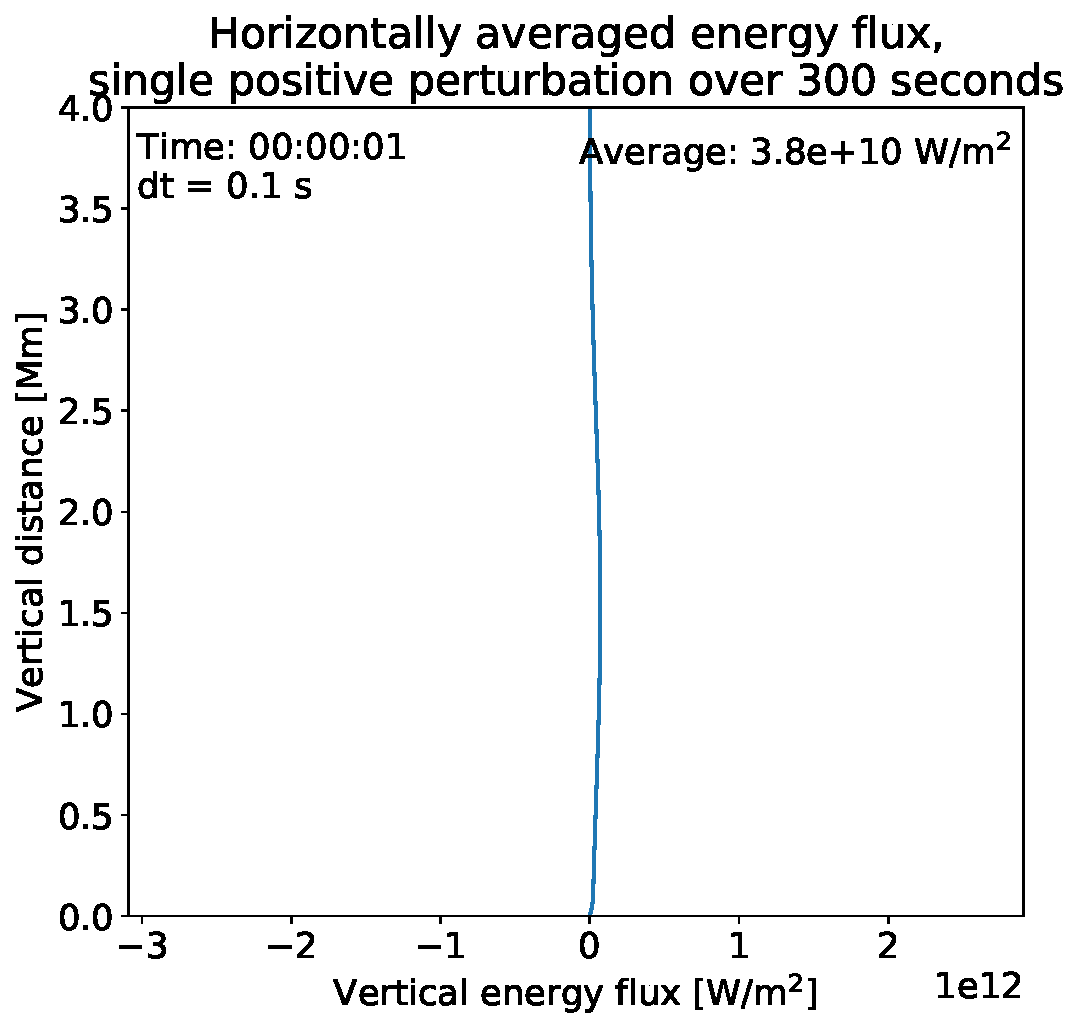
\includegraphics[width=\linewidth]{{../results/basic/snapshots/basic_endtime_300_snapshot_flux_t1.1}.pdf}
\caption{Initial situation, close to hydrostatic equilibrium.}
\label{fig:flux_t0}
\end{subfigure}
\quad
\begin{subfigure}[t]{0.45\linewidth}
\centering
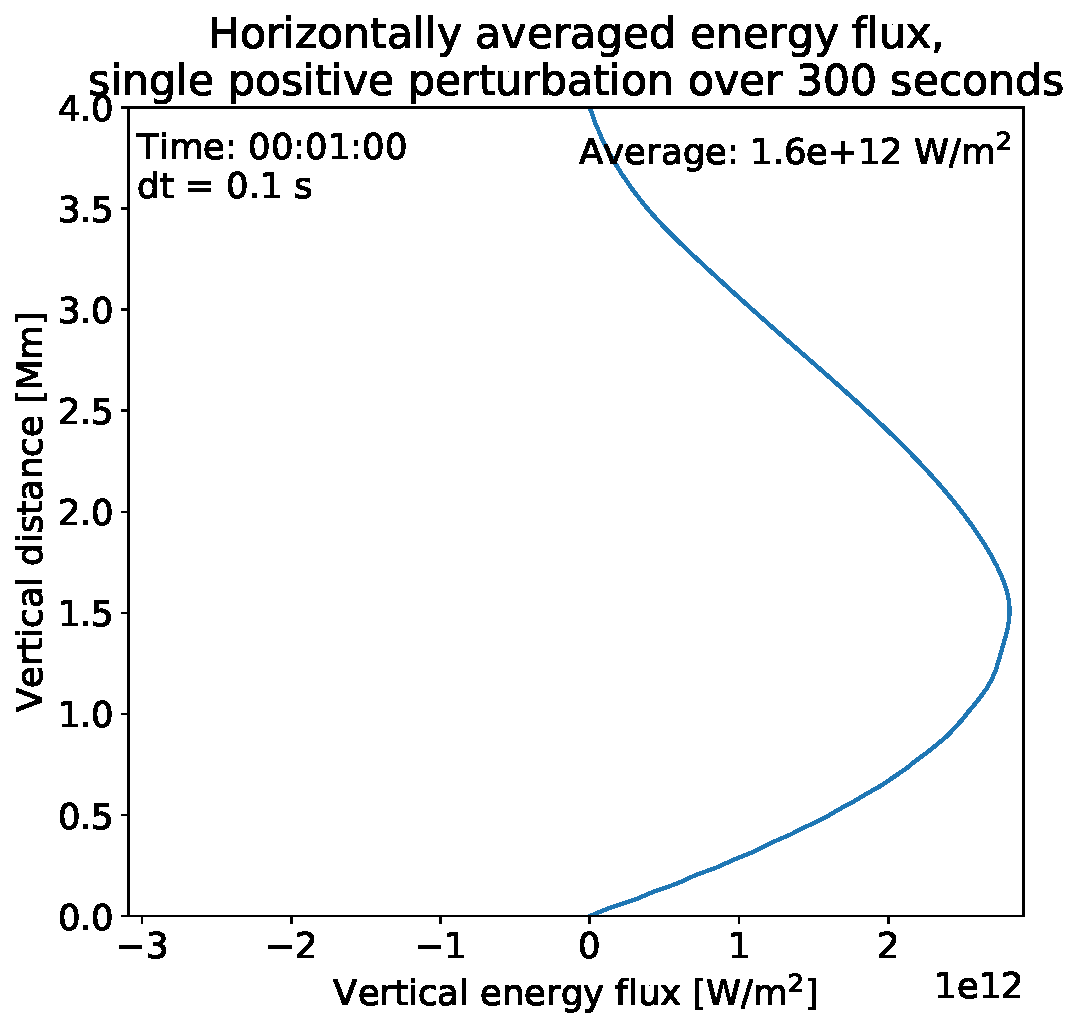
\includegraphics[width=\linewidth]{{../results/basic/snapshots/basic_endtime_300_snapshot_flux_t60.5}.pdf}
\caption{Close to the maximum of the flux, at time ${01:00}$. Consistent with what we saw in \cref{fig:Basic_t1}, here we still only have positive vertical flow, causing a large positive vertical convective flux.}
\label{fig:flux_t1}
\end{subfigure}

\vskip\baselineskip

\begin{subfigure}[t]{0.45\linewidth}
\centering
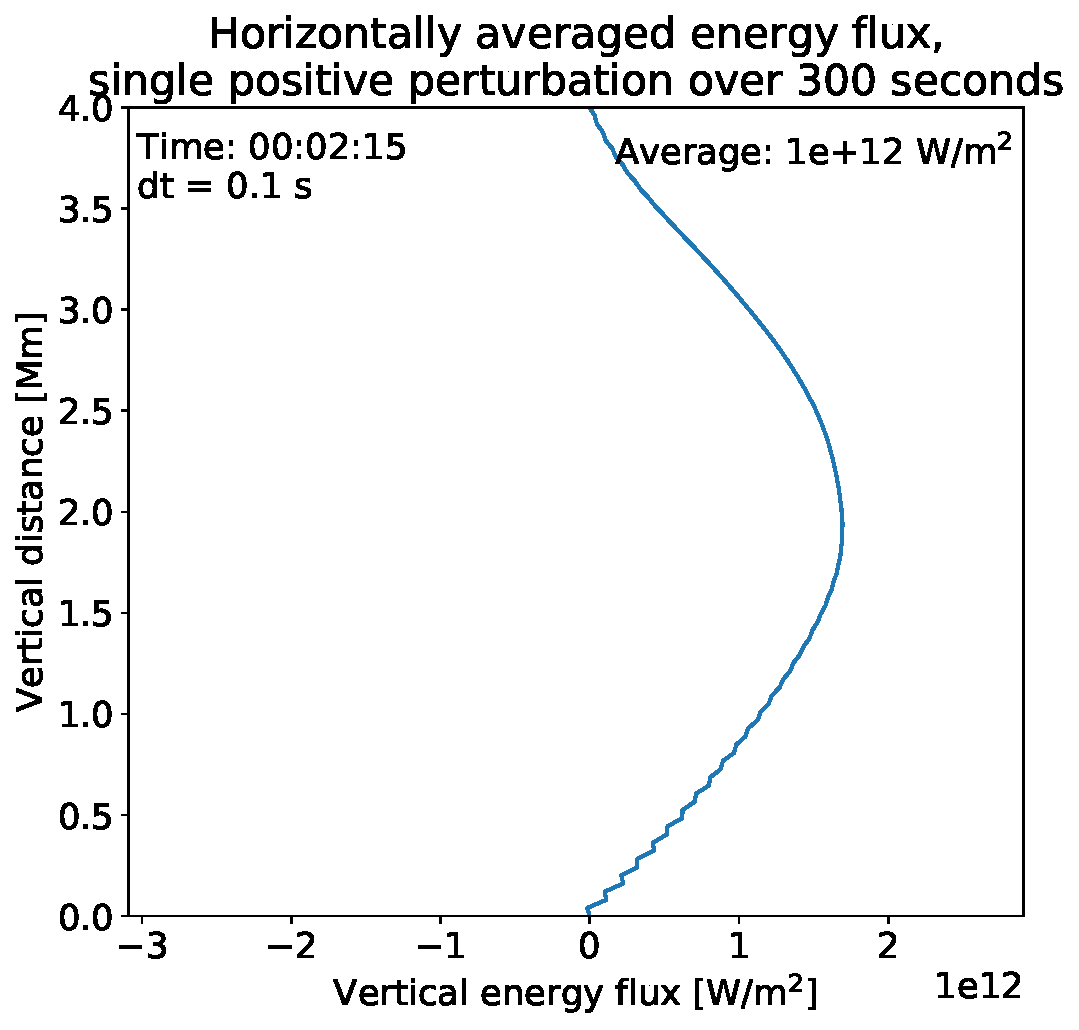
\includegraphics[width=\linewidth]{{../results/basic/snapshots/basic_endtime_300_snapshot_flux_t135.3}.pdf}
\caption{Two minutes and 15 seconds in and we see the maximum of the flux being moved to a higher $y$-value. Caused by the increase in velocity field, which increases in a circular path before it completes itself, as seen in \cref{fig:Basic_all}. Also, as the parcel rises through the medium, we get higher values of $e$ closer to the surface.}
\label{fig:flux_t2}
\end{subfigure}
\quad
\begin{subfigure}[t]{0.45\linewidth}
\centering
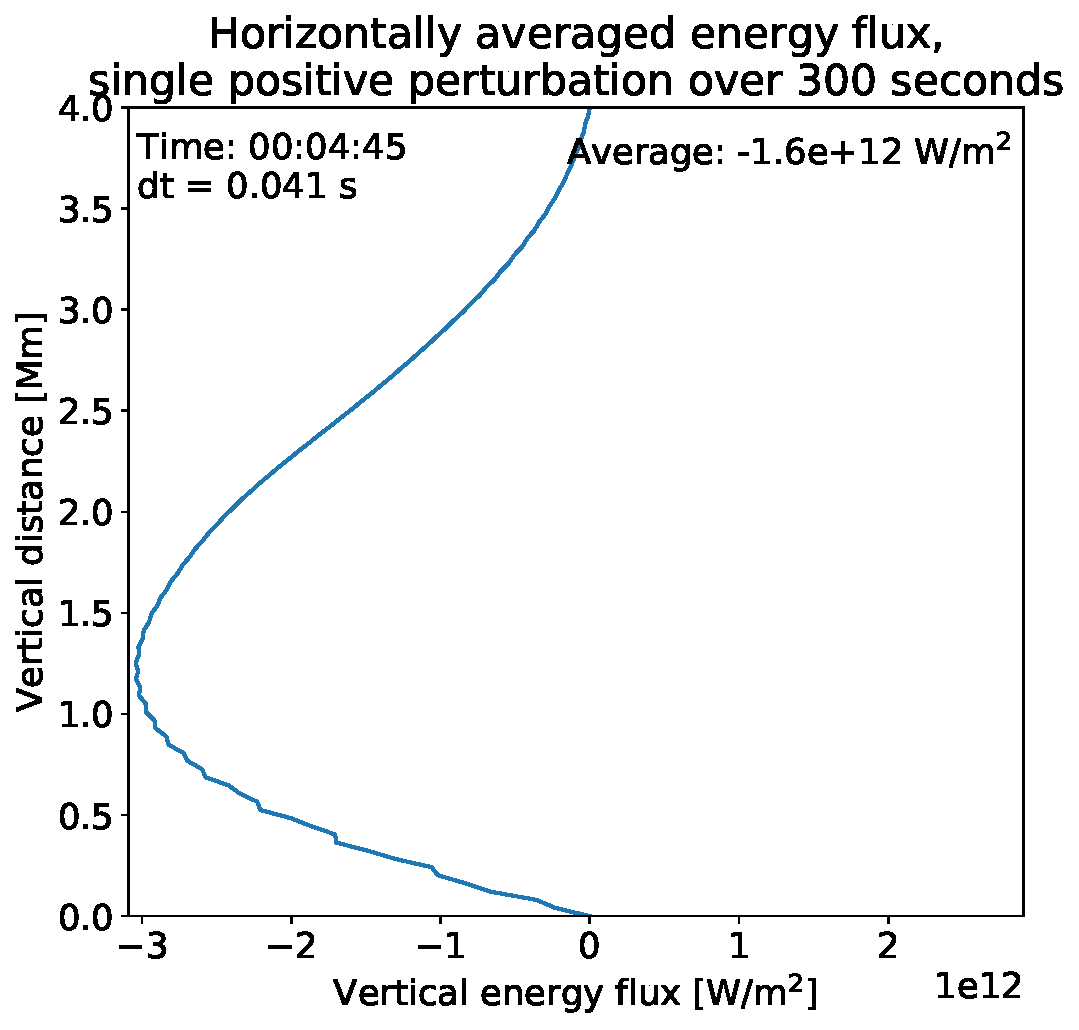
\includegraphics[width=\linewidth]{{../results/basic/snapshots/basic_endtime_300_snapshot_flux_t285.059}.pdf}
\caption{Finally we have a minimum value of the flux, being negative at all depths. This is caused by the parcel falling back down at both sides of the rising pocket. Now the areas where negative flow is happening are so much larger than the positive part, and so the averaged flux across each depth is negative.}
\label{fig:flux_t3}
\end{subfigure}

\end{figure*}
% END FLUX FIGURE

% BASIC FIGURE
\begin{figure*}
\centering
\caption{Distribution of temperature shown in colors, velocity vector field shown as arrows. \Cref{fig:Basic_t0,fig:Basic_t1,fig:Basic_t2,fig:Basic_t3} shows the time evolution of the system. Initial conditions are perturbed with a single positive circular Gaussian perturbation, which acts as a parcel of hot gas rising through the medium. The hot pocket eventually reach the surface and cools down, before it is pushed to the side and falls back down, creating a 2D convection cell. Further discussion of the results in \cref{sec:Conclusion}.}
\label{fig:Basic_all}
	\begin{subfigure}[t]{\linewidth}
	\centering
	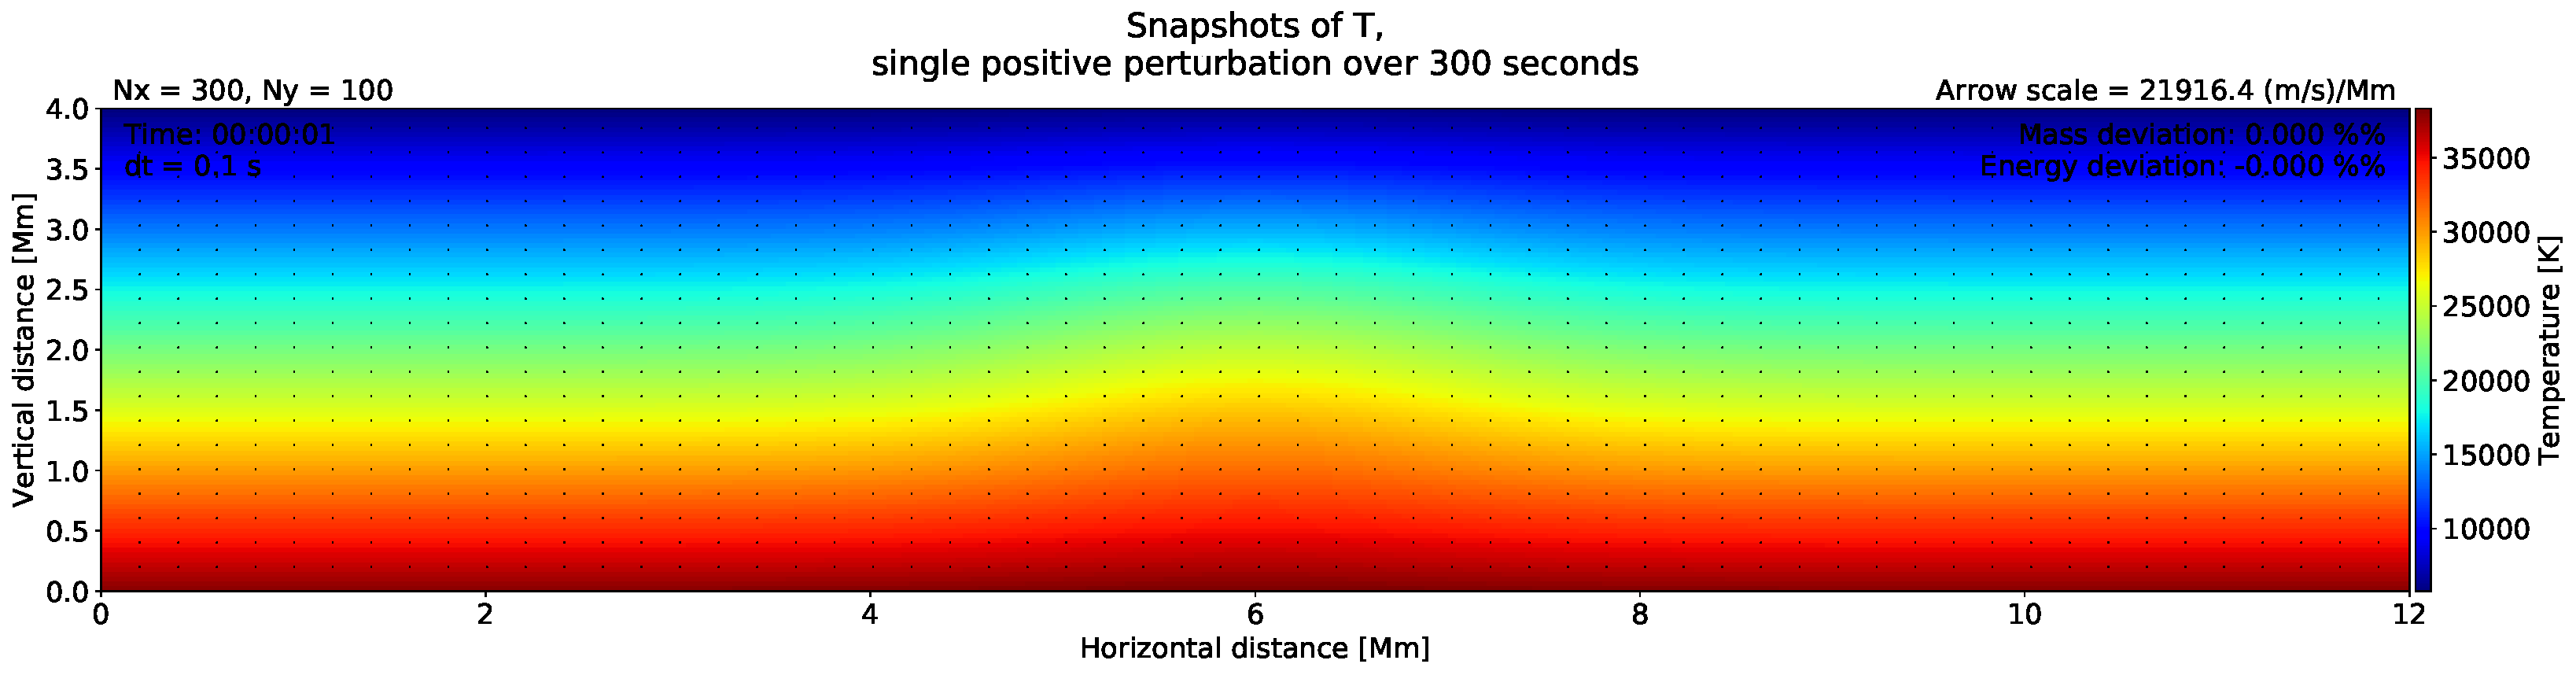
\includegraphics[width=\linewidth]{{../results/basic/snapshots/basic_endtime_300_snapshot_t1.1}.pdf}
	\caption{The initial distribution, before the perturbation give non-zero velocity. The increased temperature is visible as the bulk in the y-direction. Notice the zero (or close to zero) value of the velocity field over the hole volume.}
	\label{fig:Basic_t0}
	\end{subfigure}
	
	\begin{subfigure}[t]{\linewidth}
	\centering
	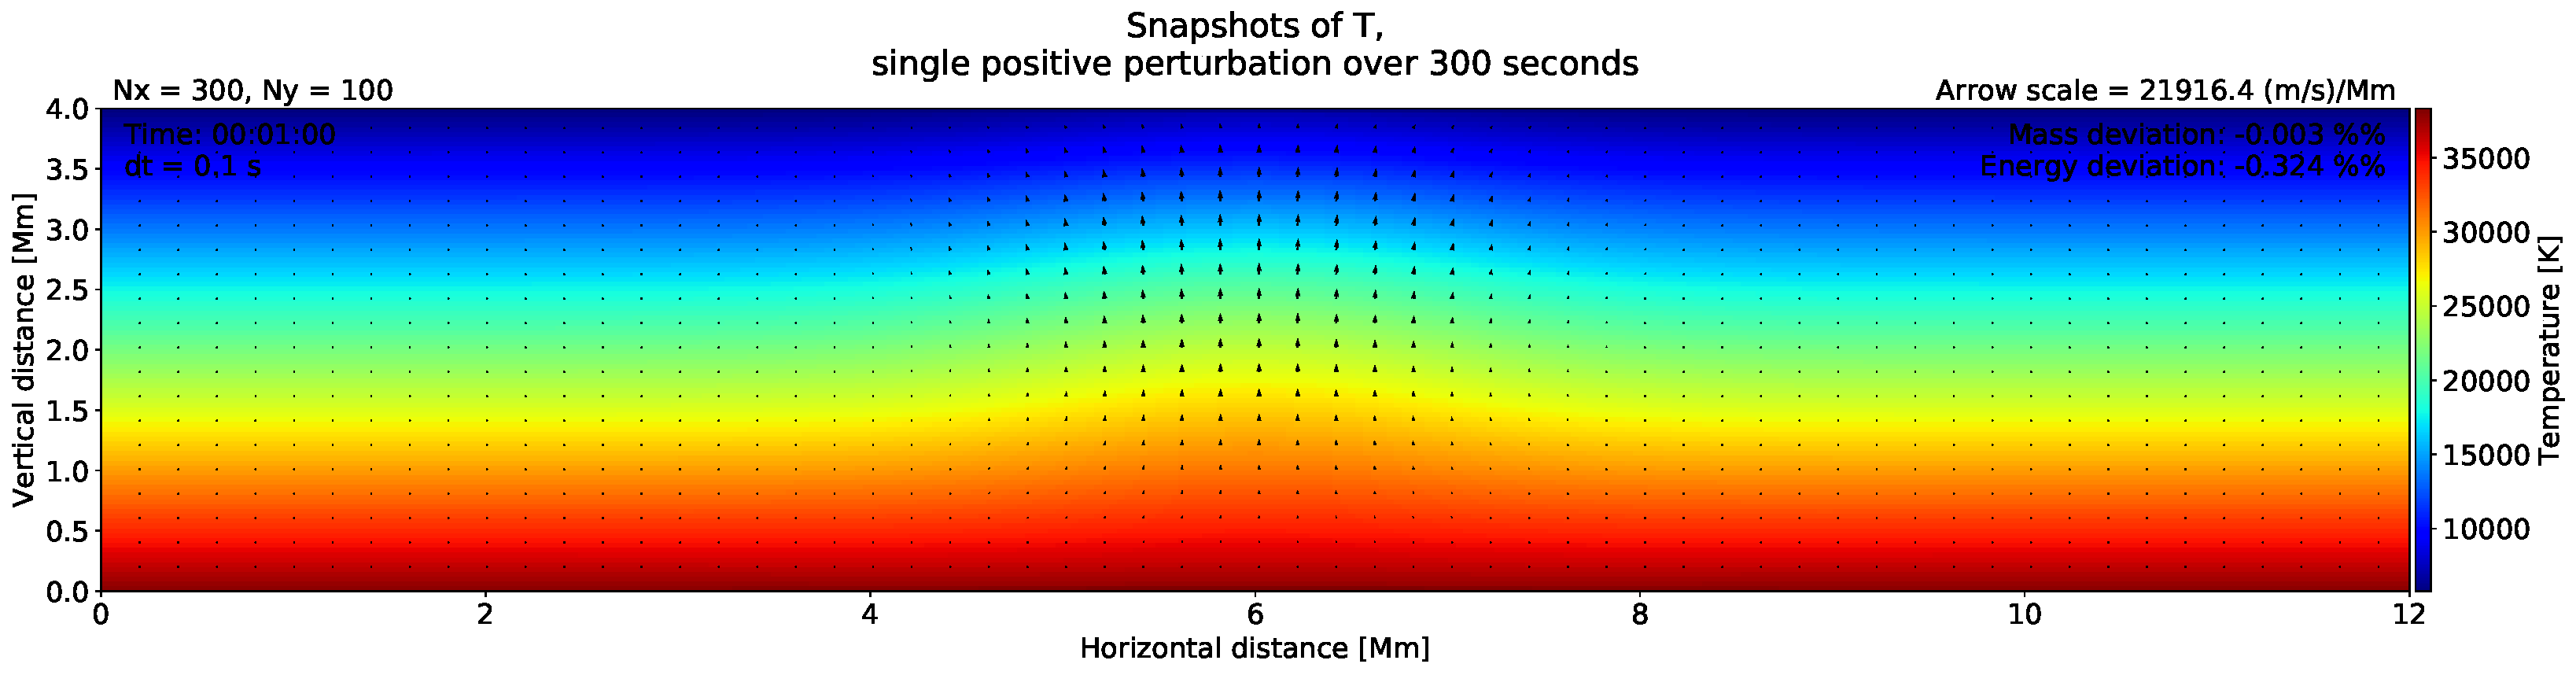
\includegraphics[width=\linewidth]{{../results/basic/snapshots/basic_endtime_300_snapshot_t60.5}.pdf}
	\caption{One minute into the simulation. Here we see the effects of the hot parcel, giving rise to positive vertical flow in the center of the box pushing the parcel towards the surface.}
	\label{fig:Basic_t1}
	\end{subfigure}

	\begin{subfigure}[t]{\linewidth}
	\centering
	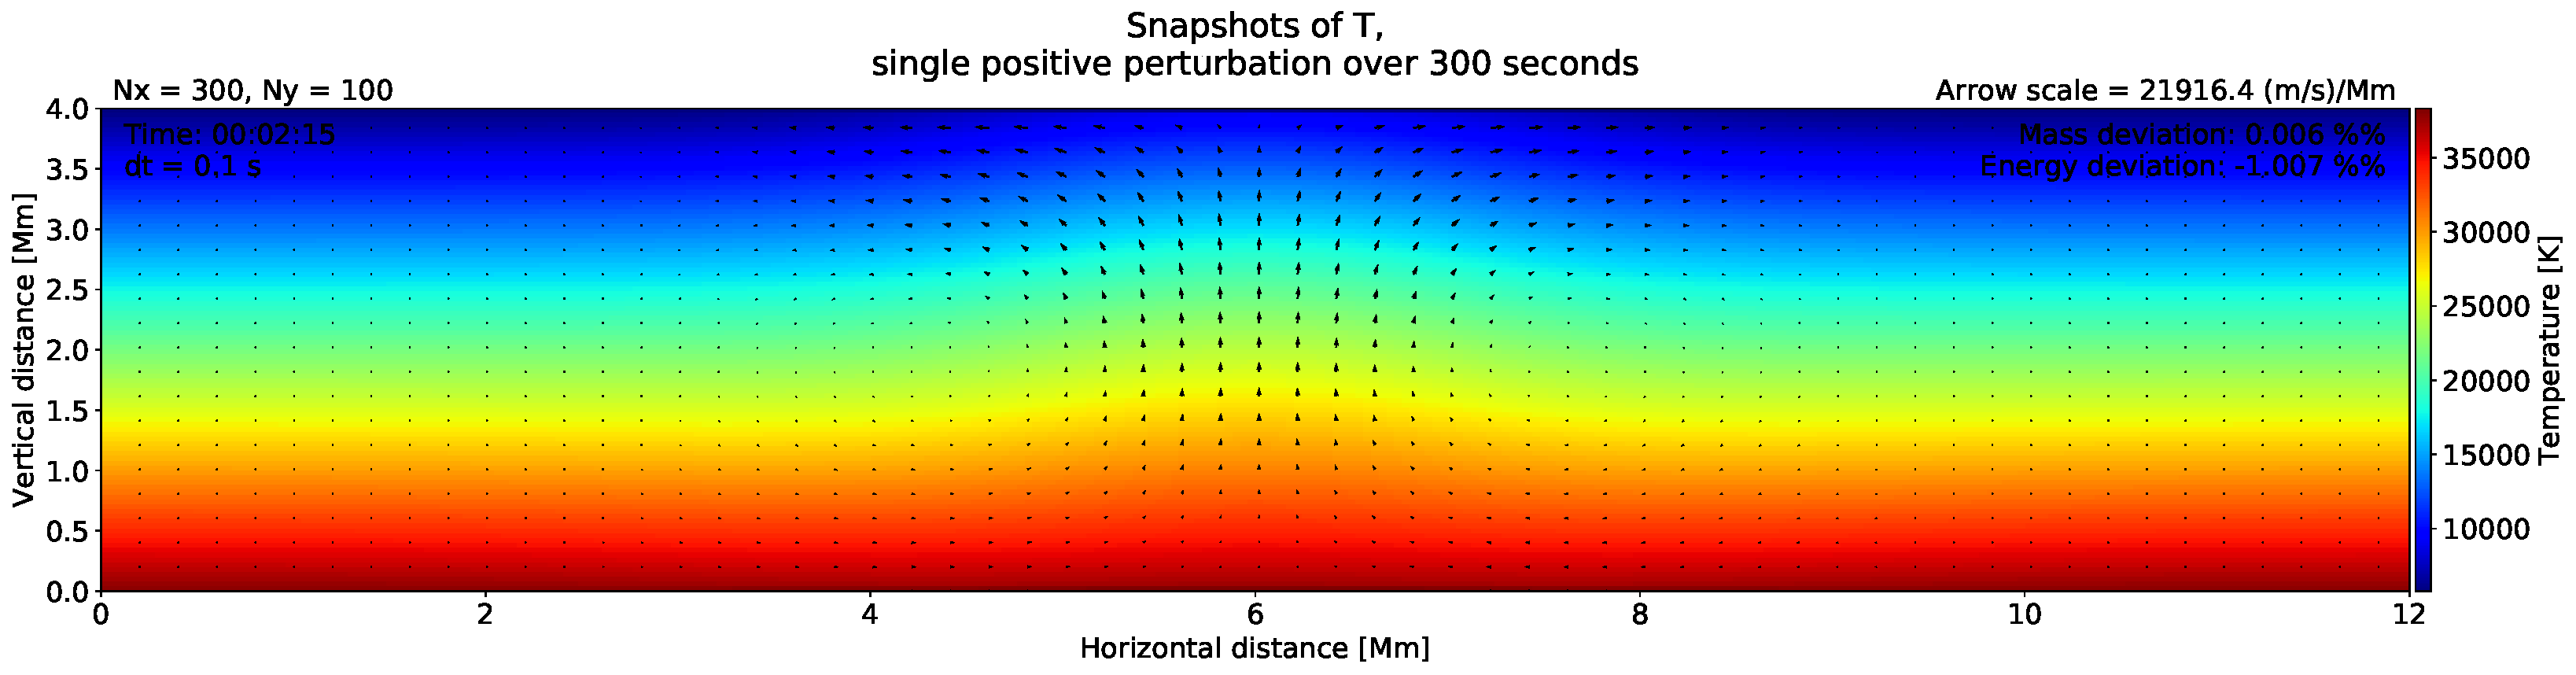
\includegraphics[width=\linewidth]{{../results/basic/snapshots/basic_endtime_300_snapshot_t135.3}.pdf}
    \caption{$02:15$ into the simulation and we can see how the medium is pushed out to each side horizontally when the parcel reaches the surface. This is as expected, as we know these can be observed as granules on the Sun.}
	\label{fig:Basic_t2}
	\end{subfigure}	
	
    \begin{subfigure}[t]{\linewidth}
	\centering
	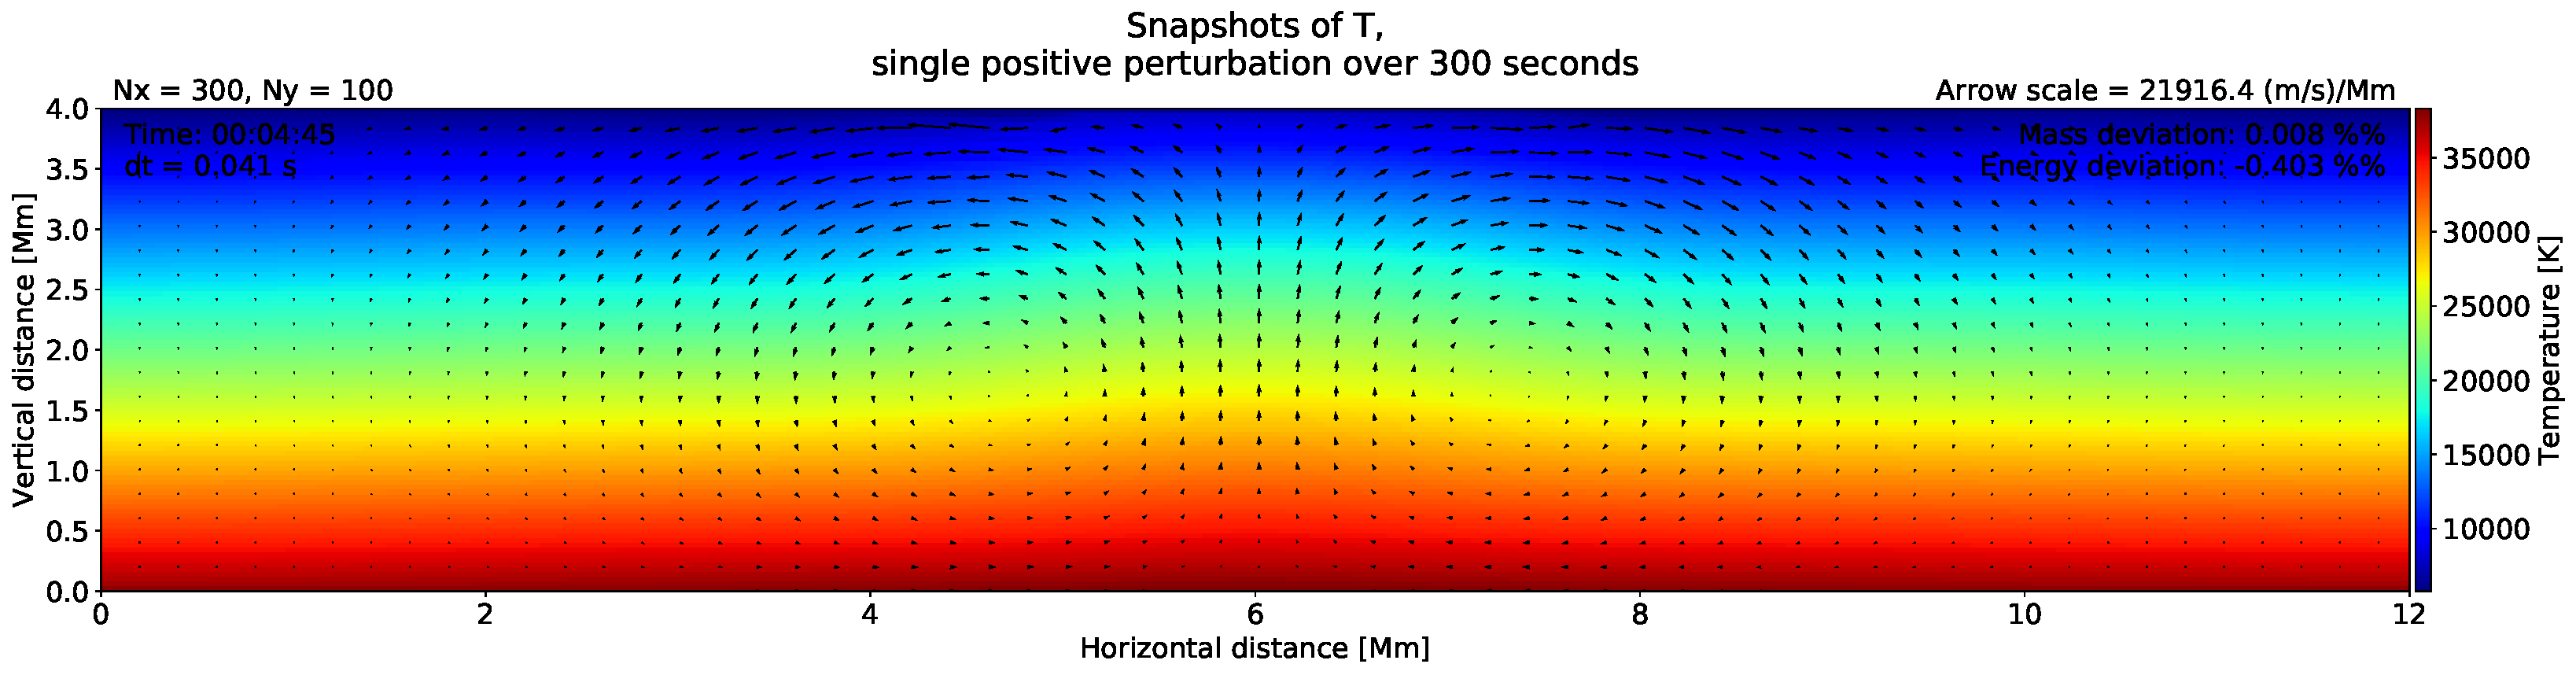
\includegraphics[width=\linewidth]{{../results/basic/snapshots/basic_endtime_300_snapshot_t285.059}.pdf}
	\caption{The last snapshot from the simulation, at $04:45$. Here we see how the cooled gas that has been pushed to the sides falls back down. This process concludes the convection <<circle>>, and is visible in the pleasant circular velocity fields at both sides of central hot rising region.}
	\label{fig:Basic_t3}
	\end{subfigure}
	
\end{figure*}
% END BASIC FIGURE

% VIZ FIGURE
\begin{figure*}
\centering
\caption{Distribution of temperature shown in colors, velocity vector field shown as arrows. \Cref{fig:viz_t0,fig:viz_t1,fig:viz_t2,fig:viz_t3} shows the time evolution of the system. Initial conditions are perturbed with 5 circular Gaussian perturbations equally spaced along x-direction, with altering sign of the perturbation. This creates both parcels rising and falling in the medium, accelerating the process of completing the convection <<circles>>. We refer to the figure captions in \cref{fig:Basic_all} and \cref{sec:Conclusion} for a more detailed discussion of the result.}
\label{fig:viz_all}
    \begin{subfigure}[t]{\linewidth}
    \centering
	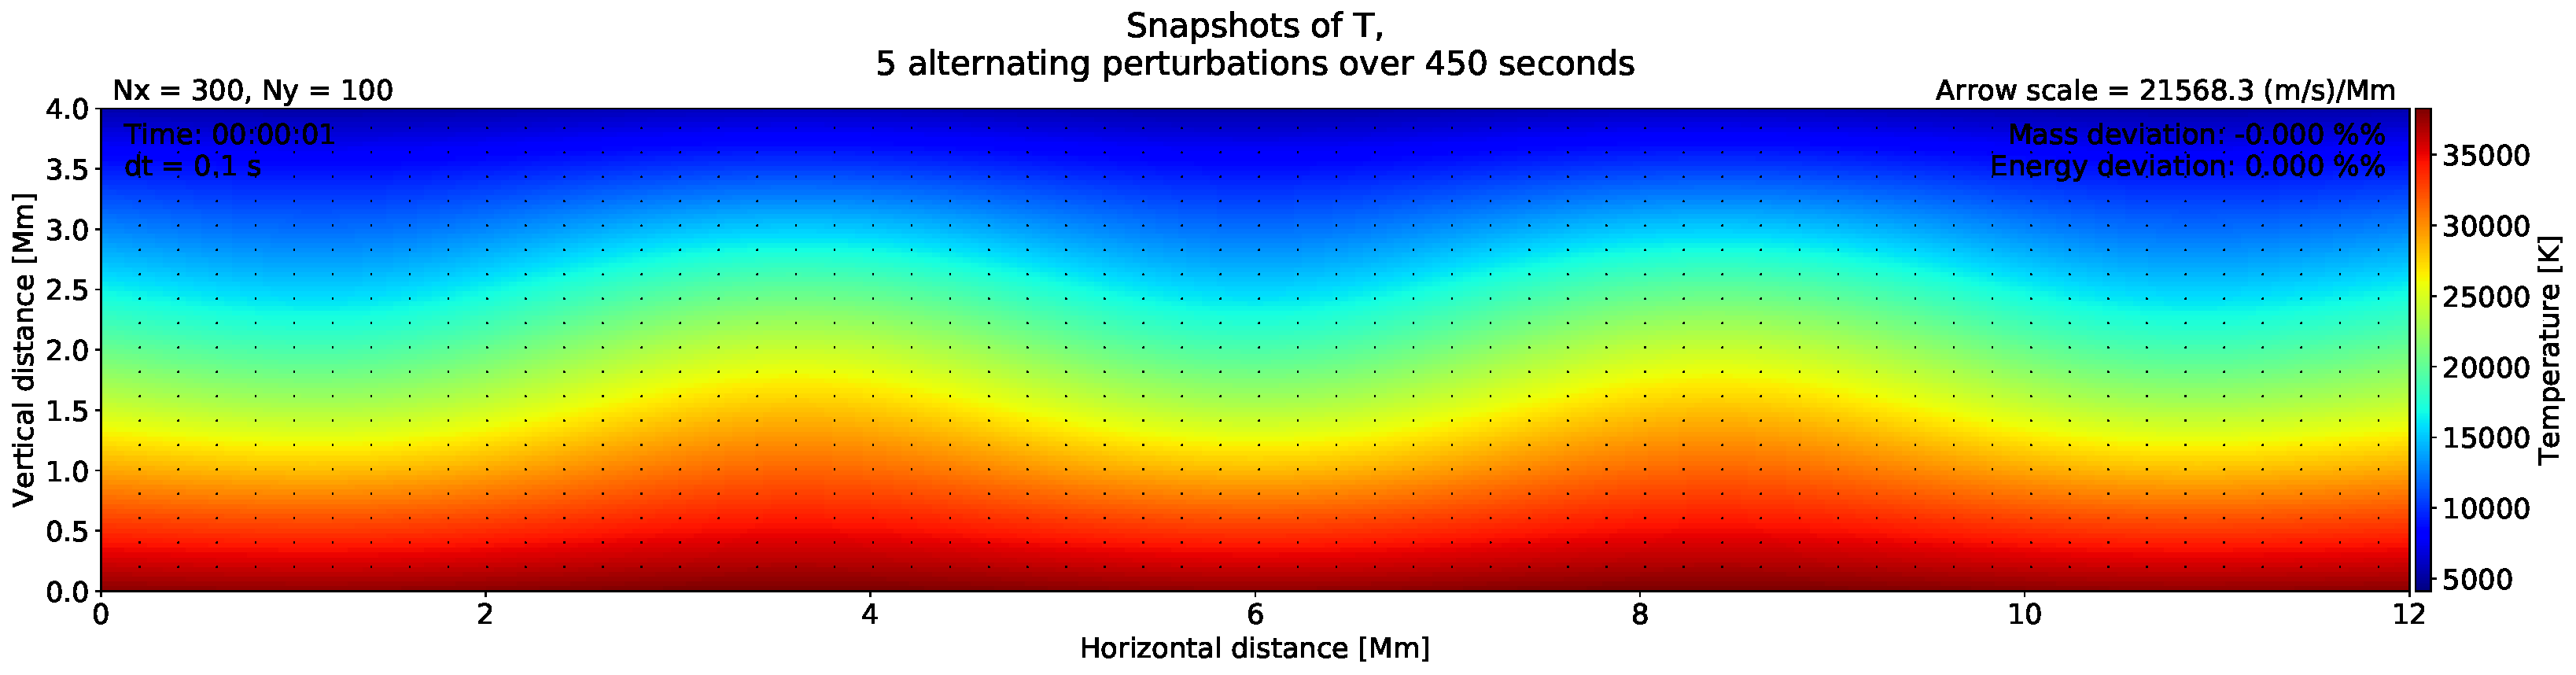
\includegraphics[width=\linewidth]{{../results/viz/snapshots/viz_5_blobs_endtime_450_snapshot_t1.3}.pdf}
	\caption{Initial temperature distribution. Compared to \cref{fig:Basic_t0} the perturbation seems larger, but that is only caused by the neighboring negative perturbation.} 
	\label{fig:viz_t0}
    \end{subfigure}
    
    \begin{subfigure}[t]{\linewidth}
    \centering
	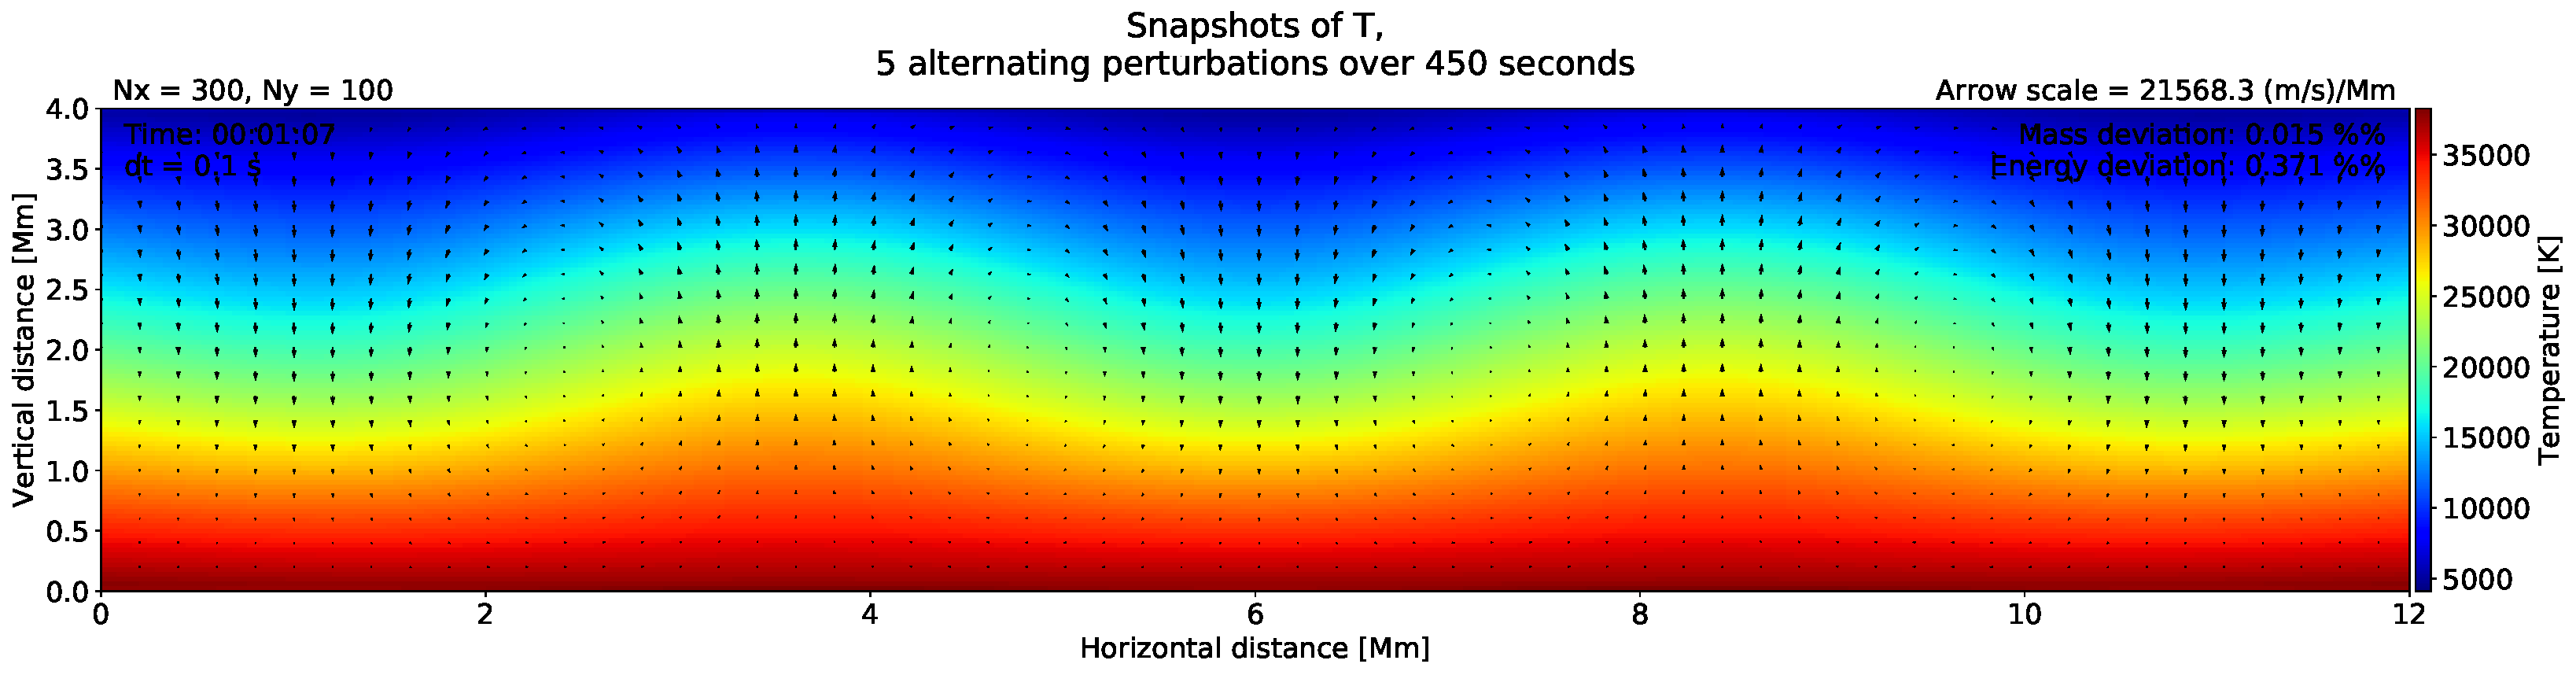
\includegraphics[width=\linewidth]{{../results/viz/snapshots/viz_5_blobs_endtime_450_snapshot_t67.6}.pdf}
	\caption{One minute and 7 seconds into the simulation and we have five rising and sinking parcels. We can see compared to \cref{fig:Basic_t1} the process of completing the convection cells are already visible.}
	\label{fig:viz_t1}
    \end{subfigure}

    \begin{subfigure}[t]{\linewidth}
    \centering
	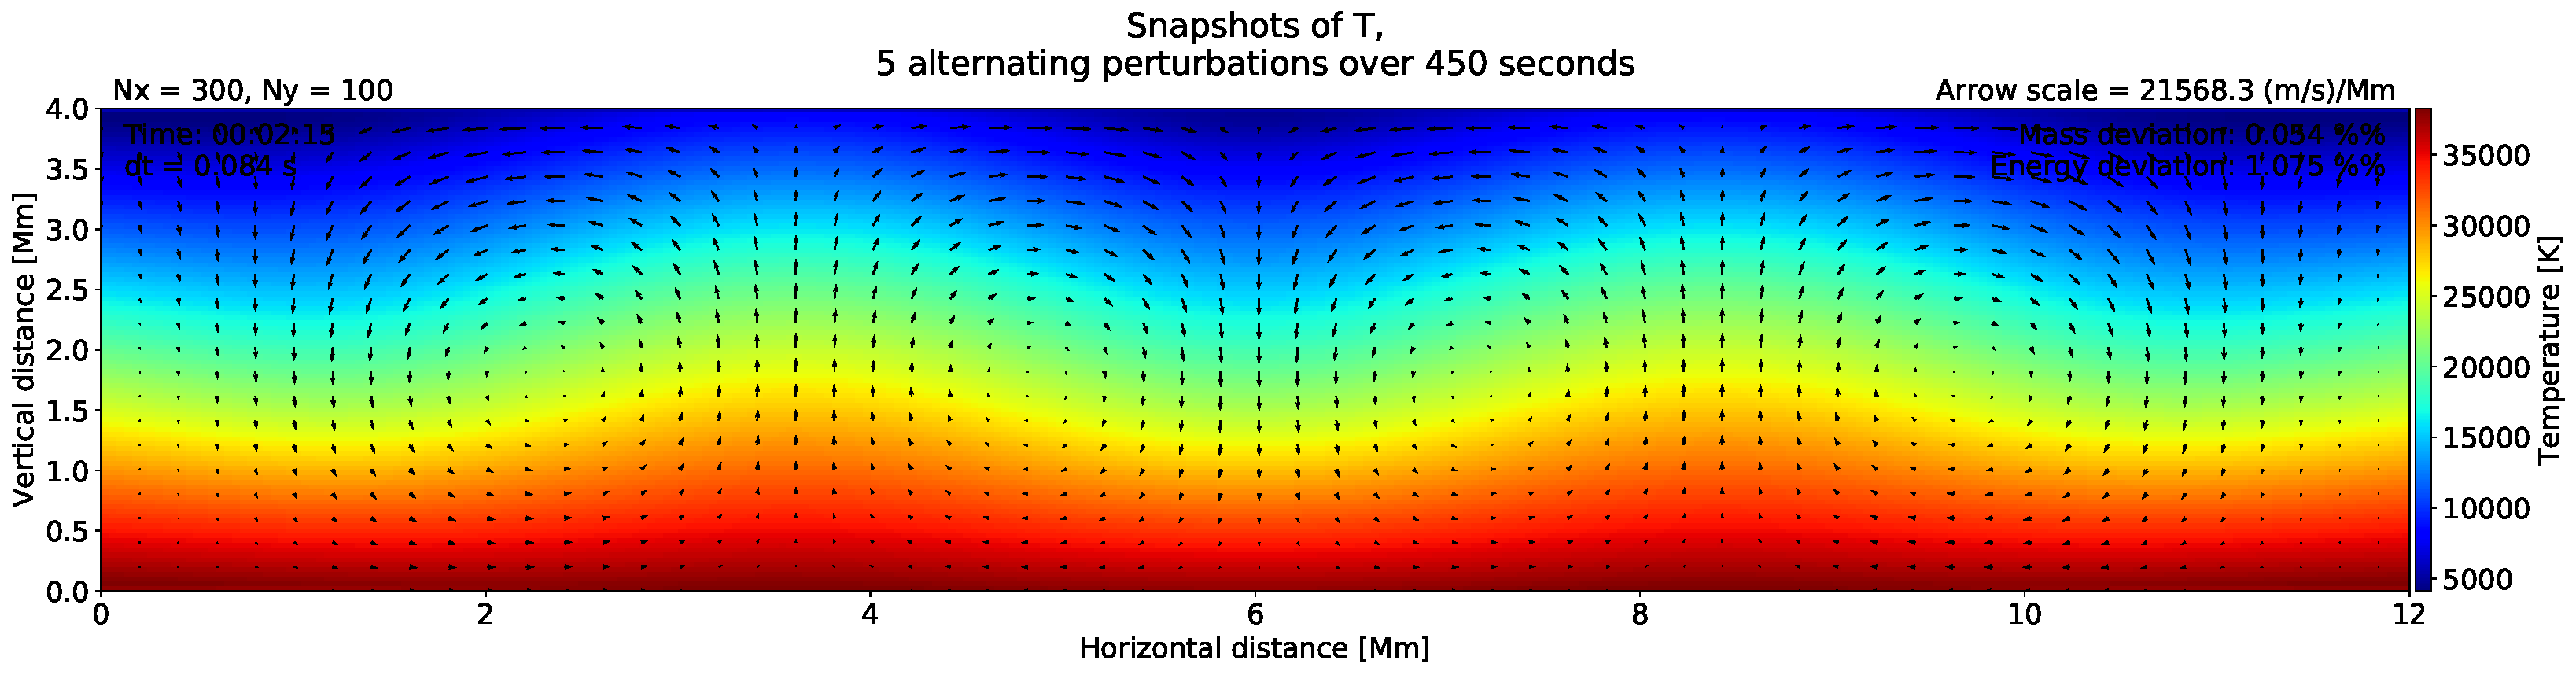
\includegraphics[width=\linewidth]{{../results/viz/snapshots/viz_5_blobs_endtime_450_snapshot_t135.1}.pdf}
	\caption{Already at two minutes and 15 seconds we can see that the convection cells are fully formed.}
	\label{fig:viz_t2}
    \end{subfigure}
    
    \begin{subfigure}[t]{\linewidth}
    \centering
	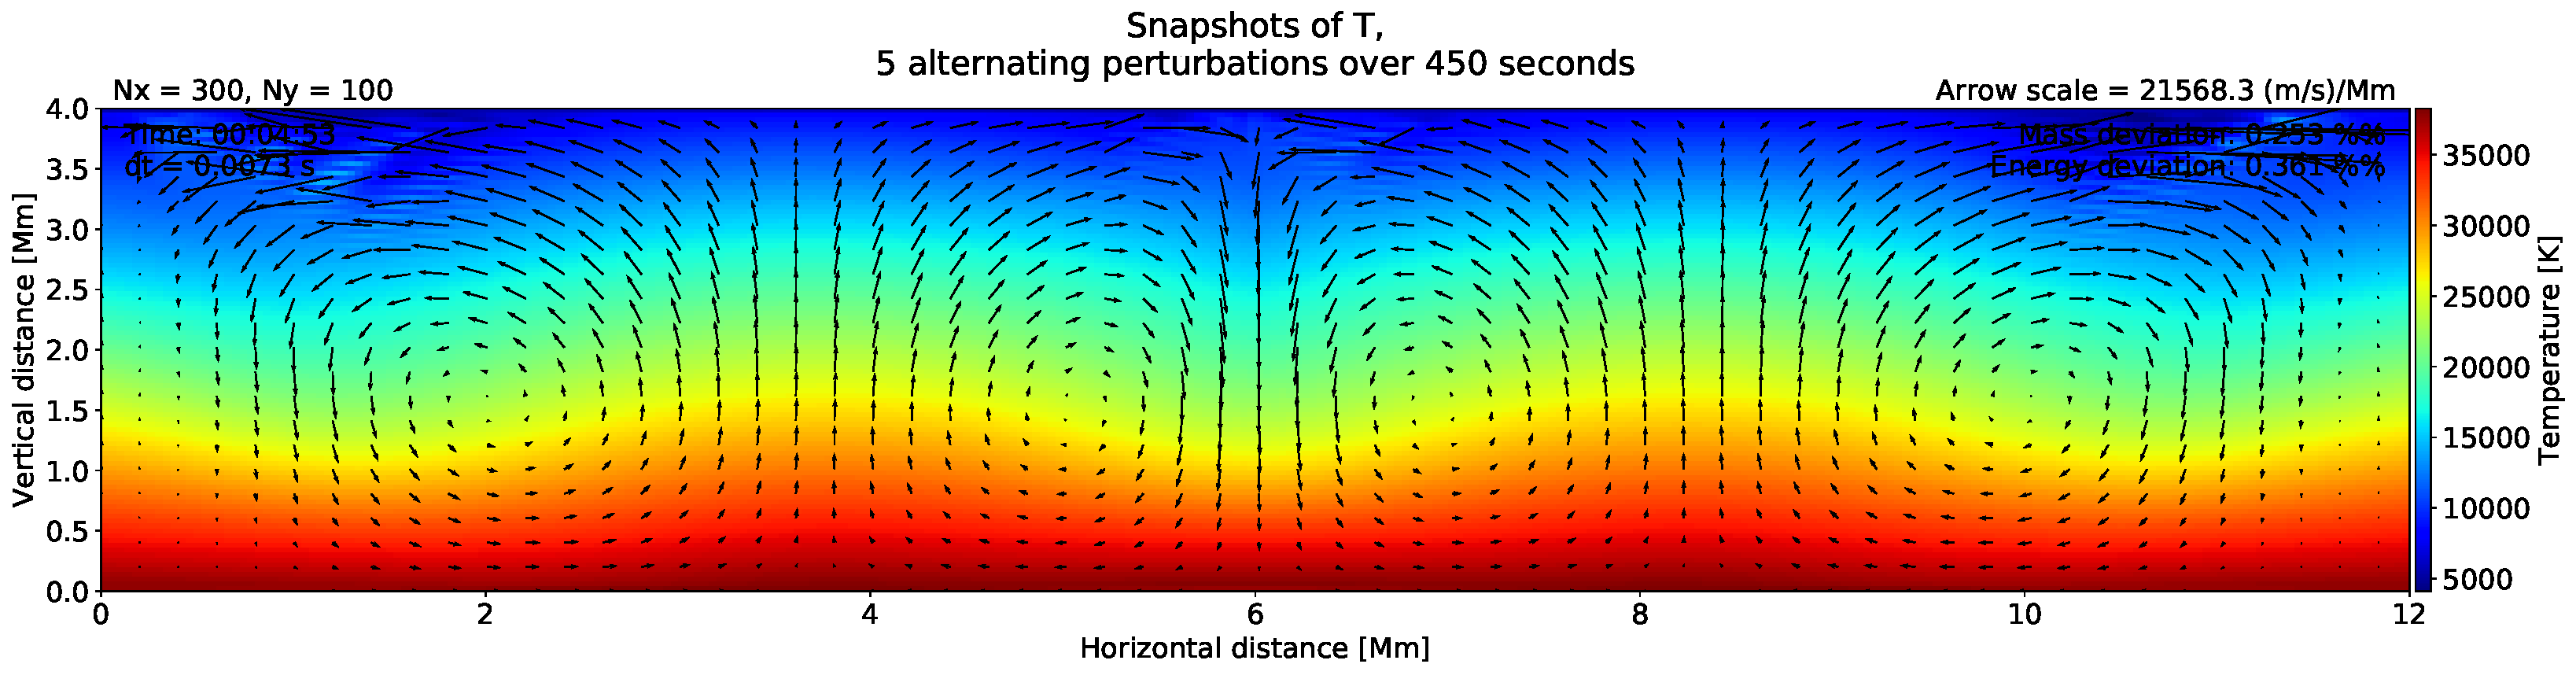
\includegraphics[width=\linewidth]{{../results/viz/snapshots/viz_5_blobs_endtime_450_snapshot_t293.482}.pdf}
	\caption{Here we show how the simulation starts to break down after a while. Unphysical behavior is present near the edges of our computational volume, especially in each corner and at the top middle area where the two rising parcels meet.}
	\label{fig:viz_t3}
    \end{subfigure}
    
\end{figure*}
% END VIZ FIGURE

\subsection{Comments, Final Thoughts and Future Perspectives}\label{subsec:Conclusion/Comments}
In this project we have successfully written a 2D hydrodynamics code, able to visualize any of the involved quantities in an informative and beautiful way. We have studied a highly unstable system of partial differential equations, and how to solve them numerically using non-trivial, but still simplistic, methods. We have also gotten new and deeper insight into how coupled all these quantities are through the equations of state. The results has helped us visualize the theory we've covered in lectures, so that we understand the simple form of 2D convection.

We have learned more about boundary conditions, and how important they are for confined systems like this. The process of finding the correct boundary conditions were interesting and challenging, as we had little information to go on. This forced us to do a lot of healthy critical physical thinking. Also being able to test how slightly different \textit{wrong} boundaries changed the behavior of the system was educational.

We've had few problems all in all. That doesn't say the different parts of the project haven't been difficult, but in a good way. Our biggest issue was in the very beginning of the project, whit a lot of information about the system and the problem to absorb. Here we had to figure out how to orient the system and the model in a physically, a numerical and a graphical sense. Through the direction of gravity and the vertical pressure gradient we established how the situation had to behave physically, and then translated that into numerical indexation in Python. Lastly we had to think about how this was handled by the provided visualization module, which flips the vertical axis. After obtaining good understanding of these concepts the rest of the project became much easier. It was then just a matter of writing the code in an ordered fashion, utilizing modules for as much as possible. After the full implementation was complete, following \cref{subsec:Method/Benchmarks}, the simulation worked as intended surprisingly fast with little to no bugs.

As mentioned our model is not complete, as we are not able to simulate turbulence. This could be improved by including the viscous stress tensor in our governing equation for the momentum. The stress tensor governs internal friction in the dynamical system. The friction is present between neighboring flow streams of mass with different velocities. We can see how our current simulations struggles with this near the edges where the boundary conditions creates shock waves of unphsycial behavior, and where there are large relative differences in the velocity field over small areas as seen \cref{fig:viz_t3}. In addition we could include diffusion, as we know from the density gradient there should be some contribution from diffusion in our dynamical system. These inclusions are not trivial however, and would probably require some higher ordered numerical solvers. We could also have implement higher order solvers, both temporal and spatial, without the tensor or diffusion. If so the simulations would probably stay stable for longer, as especially the central differential method is unconditionally unstable.

\vspace{0.2 cm}
\noindent
\textbf{\large Acknowledgments}

The author would like to thank Helle Bakke and Boris Vilhelm Gudiksen for an exciting and interesting course, with some inspiring lectures and projects. Thanks to my colleagues for discussions during all the terms projects, in particular Jon Kristian Dahl, Bernhard Nornes Lotsberg, Mats Ola Sand, Nils-Ole Strutzer and Håkon Tansem.
\vspace{0.2cm}

\bibliography{ref3}

\end{document}
